% --- UNIVERSAL PREAMBLE BLOCK ---
\documentclass[11pt, a4paper]{article}
\usepackage[a4paper, top=2.5cm, bottom=2.5cm, left=2.5cm, right=2.5cm]{geometry} % More balanced margins

% pdfLaTeX compatible language and font setup
\usepackage[english]{babel}
\usepackage[sfdefault]{noto}
\usepackage{microtype} % Added for better typography/justification

% --- ADDITIONAL PACKAGES ---
\usepackage{graphicx}    % Added for Directive A image fallback
\usepackage{float}       % Required for [H] float placement specifier
\usepackage{tabularx}    % For flexible width tables
\usepackage{booktabs}    % For professional table rules
\usepackage{parskip}     % For better paragraph spacing without indents
\usepackage{enumitem}    % For list customization
\usepackage{xcolor}      % Added for professional color accents
\usepackage{titlesec}    % Added for beautiful section headers
\usepackage{fancyhdr}    % Added for professional page headers and footers
\usepackage{hyperref}    % For clickable links and TOC (Must be last)

% --- GLOBAL STYLING ---
% Define brand colors
\definecolor{PrimaryColor}{HTML}{003A70} % Corporate Blue
\definecolor{SecondaryColor}{HTML}{555555} % Dark Gray

% Configure hyperref to look clean
\hypersetup{
    colorlinks=true,
    linkcolor=PrimaryColor,
    filecolor=magenta,      
    urlcolor=PrimaryColor,
    citecolor=PrimaryColor,
    pdftitle={Software Requirements Specification},
    pdfpagemode=FullScreen,
}

% Section styling
\titleformat{\section}
  {\color{PrimaryColor}\normalfont\Large\bfseries}
  {\thesection}{1em}{}[\vspace{-0.5em}\rule{\textwidth}{0.5pt}]
\titleformat{\subsection}
  {\color{PrimaryColor}\normalfont\large\bfseries}
  {\thesubsection}{1em}{}
\titleformat{\subsubsection}
  {\color{PrimaryColor}\normalfont\normalsize\bfseries}
  {\thesubsubsection}{1em}{}

% Header and Footer configuration
\pagestyle{fancy}
\fancyhf{}
\fancyhead[L]{\color{SecondaryColor}\small Software Requirements Specification}
\fancyhead[R]{\color{SecondaryColor}\small AFSMS v1.0}
\fancyfoot[L]{\color{SecondaryColor}\small Automated Faculty Student Management System (AFSMS) v1.0}
\fancyfoot[R]{\color{SecondaryColor}\thepage}
\renewcommand{\headrulewidth}{0.4pt}
\renewcommand{\footrulewidth}{0.4pt}

% Table and List spacing
\renewcommand{\arraystretch}{1.3} % More breathable tables
\setlist[itemize]{itemsep=0.2em, topsep=0.2em} % Tighter, cleaner lists
\setlist[enumerate]{itemsep=0.2em, topsep=0.2em}

\begin{document}

% --- TITLE PAGE ---
\begin{titlepage}
    \begin{center}
        \vspace*{1cm}
        
        \textcolor{PrimaryColor}{\rule{\textwidth}{1.5pt}}\vspace{0.5cm}
        
        {\Huge \bfseries \textcolor{PrimaryColor}{Software Requirements Specification}} \\[0.5cm]
        {\Large \textit{for}} \\[0.5cm]
        {\LARGE \bfseries Information System for the} \\
        {\LARGE \bfseries Automatic Management of Faculty Students}
        
        \vspace{0.5cm}\textcolor{PrimaryColor}{\rule{\textwidth}{1.5pt}}
        
        \vspace{1.5cm}
        {\Large \textbf{Version:} 1.0 approved}
        
        \vfill
        
        \begin{flushleft}
            {\Large \textbf{Prepared by:}} \\[0.3cm]
            {\large Sugubete Andrei} \\
            {\large Maximilian Andrei} \\
            {\large Mitrache Marian Nicușor}
        \end{flushleft}
        
        \vspace{1.5cm}
        
        \begin{flushright}
            {\Large \textbf{University of Craiova}} \\[0.2cm]
            {\large Faculty of Automation, Computers and Electronics} \\[0.2cm]
            {\large \textbf{Date:} 07.03.2026}
        \end{flushright}
        
        \vspace{2cm}
        \rule{\textwidth}{0.5pt}\vspace{0.2cm}
        
        \footnotesize \textcopyright\ 1999 by Karl E. Wiegers. Permission is granted to use, modify, and distribute this document.
    \end{center}
\end{titlepage}

% --- TABLE OF CONTENTS ---
\tableofcontents
\newpage

% --- REVISION HISTORY ---
\section*{Revision History}
\addcontentsline{toc}{section}{Revision History}

\begin{table}[htbp]
\centering
\begin{tabularx}{\textwidth}{l l X l}
\toprule
\textbf{Name} & \textbf{Date} & \textbf{Reason For Changes} & \textbf{Version} \\
\midrule
Everyone & 23.02.2026 & Init. Made work on 1.x and 2.x. & 0.1 \\
\midrule
Sugubete Andrei & 27.02.2026 & Added TODO's for better workflow. Reviewed 1.1., 1.4., 2.1., 2.3, 2.4. Did 2.3., 2.5., 2.6., 2.7. & 0.2 \\
\midrule
Mitrache Marian & 27.02.2026 & Did 1.3 and added a new user at 2.3 (TESTER), 1.5. Trecand prin ce este de la 3 incolo trebuie sa facem impreuna. Reviewed 1.3, 1.5. & 0.3 \\
\midrule
Everyone & 07.03.2026 & Finishing up: Final review and formatting for submission. & 1.0 \\
\bottomrule
\end{tabularx}
\end{table}

\newpage

% --- SECTION 1: INTRODUCTION ---
\section{Introduction}

\subsection{Purpose}
This Software Requirements Specification (SRS) describes the functional and non-functional requirements for Version 1.0 of the Automated Faculty Student Management System (AFSMS). It covers how AFSMS will manage curricula, student records, and document workflows to digitalize the faculty's administrative processes.

The document serves as the primary technical reference for the development team, QA testers, project managers, and university stakeholders (secretariat staff and faculty).

\subsection{Document Conventions}
\begin{itemize}
    \item \textbf{Headings:} Times New Roman, size 14, bold (per the document template).
    \item \textbf{Body text:} Arial, size 11.
    \item ``Shall'' indicates mandatory behavior; ``should'' indicates recommended behavior.
    \item Functional requirements use IDs REQ-XX, non-functional requirements use NFR-XX.
    \item \textbf{Bold} text highlights key terms when first introduced.
\end{itemize}

\subsection{Intended Audience and Reading Suggestions}
Each audience should prioritize sections relevant to their role:
\begin{itemize}
    \item \textbf{Registrar and Secretariat Staff (Primary):} Section 2.2 (Product Functions) and Section 3.1 (User Interfaces).
    \item \textbf{External Visitors and Prospective Students:} Section 2.2 and Section 3.1.1 (Public Web Interface).
    \item \textbf{Software Developers and Architects:} Section 3 (External Interface Requirements) and Section 4 (System Features).
    \item \textbf{System Administrators:} Section 5.2 (Safety) and Section 5.3 (Security).
    \item \textbf{Academic Staff (Professors):} Section 2.2 and Section 3.1 for grade entry and communication features.
    \item \textbf{QA and Testing Teams:} Section 3 for verifiable requirements and Section 6 for testing mandates.
\end{itemize}

\subsection{Product Scope}
The product is the Automated Faculty Student Management System (AFSMS / GASF).

\textbf{Objectives and Benefits}

AFSMS automates the faculty's manual administrative workflows. Key benefits:
\begin{itemize}
    \item Eliminates data redundancy and manual entry errors via client-side validation and centralized database management.
    \item Reduces processing time for generating official documents (e-Transcript, e-Grade Centralizer).
    \item Provides 24/7 information access for students and staff via a secure, role-based web portal.
\end{itemize}

\textbf{What the System Will Do}

AFSMS provides web-based tools for:
\begin{itemize}
    \item Academic data collection and student record management.
    \item Advanced document search and filtering.
    \item Secure electronic document circulation within the secretariat.
    \item Report generation, exportable in CSV, XML, XLS, and PDF formats.
    \item Integration with Microsoft Excel and Microsoft Outlook.
    \item Activity logging, offline backups, and point-in-time database recovery (rollback).
\end{itemize}

\textbf{What the System Will Not Do}

AFSMS will not:
\begin{itemize}
    \item Process financial transactions or manage tuition fees.
    \item Interface with central HR or payroll systems.
    \item Replace institutional systems outside its academic scope.
\end{itemize}

\subsection{References}
\begin{itemize}
    \item IEEE Std 830-1998, IEEE Recommended Practice for Software Requirements Specifications.
    \item University of Craiova (ACE), Academic Curricula and Educational Plans: \url{https://ace.ucv.ro/invatamant/didactica/planuri.php}
    \item University of Craiova (ACE), Student Formations and Timetable Schedules: \url{https://ace.ucv.ro/invatamant/utile/orar.php}
    \item University of Craiova (ACE), Institutional Evaluation and Grading Procedures: \url{https://ace.ucv.ro/invatamant/utile/modalitati_de_evaluare.php}
    \item Microsoft Corporation, Microsoft Graph API Documentation for Excel and Outlook Integration.
    \item IEEE Std 610.12-1990, IEEE Standard Glossary of Software Engineering Terminology.
\end{itemize}


% --- SECTION 2: OVERALL DESCRIPTION ---
\section{Overall Description}

\subsection{Product Perspective}
AFSMS is a new, standalone software product. It provides faculty-level academic management but is not a component of any larger institutional system --- it will not replace the university's financial or HR systems.

\subsubsection{System Interfaces}
AFSMS operates independently at the registrar's office level, with minimal interfaces to higher-level university systems. It exchanges data through standardized imports and exports, focusing strictly on faculty-level workflows.

\subsubsection{User Interfaces}
\begin{itemize}
    \item \textbf{Logical characteristics:} The interface displays in a web browser with two perspectives (public and private). Screens use tabular layouts for grade registers and summaries, consistent navigation menus, and help/search functions.
    \item \textbf{Optimization:} The interface uses selection lists (dropdowns) extensively to reduce errors and increase speed.
    \item \textbf{Verifiable usability:} The system should allow rapid generation of grade summaries after minimal staff training.
\end{itemize}

\subsubsection{Hardware Interfaces}
\begin{itemize}
    \item \textbf{Server:} The physical or virtual server architecture must support concurrent processing.
    \item \textbf{Client:} No special hardware is required. Any internet-connected device (desktop PC, laptop, or tablet) with an up-to-date web browser is supported.
\end{itemize}

\subsubsection{Software Interfaces}
The system integrates with:
\begin{itemize}
    \item \textbf{RDBMS:} Stores student data and activity logs; supports web-based administration and offline backups.
    \item \textbf{Microsoft Excel (.XLS/.CSV):} Bidirectional bulk data import and report export.
    \item \textbf{Microsoft Outlook (SMTP / Microsoft Graph API):} Group messaging and document workflow communications.
\end{itemize}

\subsubsection{Communications Interfaces}
All data transfer uses HTTPS over standard ports, encrypting academic and authentication data (SSO) in transit between browser and server.

\subsubsection{Memory Constraints}
Server-side storage must be scalable to accommodate large volumes of historical data (spanning years of study) and comprehensive operation logs required for the rollback function.

\subsubsection{Operations}
\begin{itemize}
    \item \textbf{Interactive:} Grade entry, student queries, and document management during office hours.
    \item \textbf{Unattended:} Automatic offline database backups (preferably outside peak hours).
    \item \textbf{Special:} Administrator-triggered rollback and point-in-time recovery for data corruption or major errors.
\end{itemize}

\subsubsection{Site Adaptation Requirements}
The system must support faculty-specific configuration before first use, including pre-configured curricula, department types, local grading rules, and academic year structures (grid values).

\subsection{Product Functions}
AFSMS automates student management and administrative workflows through the following functions:
\begin{itemize}
    \item \textbf{Data Collection:} Gather curricula, study formations, and student records.
    \item \textbf{Data Management:} Centralized administration of academic information; data extraction from databases, Excel files, and text files.
    \item \textbf{Report Generation:} Produce official documents (e-Transcript, e-Grade Centralizer) in CSV, XML, XLS, and PDF.
    \item \textbf{Document Workflow Management:} Electronic circulation of documents within the registrar's office for information, approvals, or modifications.
    \item \textbf{Querying and Search:} Locate documents and data by file type, creation date, author, or content, using selection lists for easy navigation.
    \item \textbf{Web Portal:} Differentiated access via public and private perspectives; registered users can modify data or generate reports based on their privileges.
    \item \textbf{Logging and Data Recovery:} Record all operations in a log file; support data rollbacks to prevent collection errors.
\end{itemize}

\begin{figure}[htbp]
    \centering
    \framebox{\parbox{0.85\textwidth}{\centering
      \vspace{0cm}
      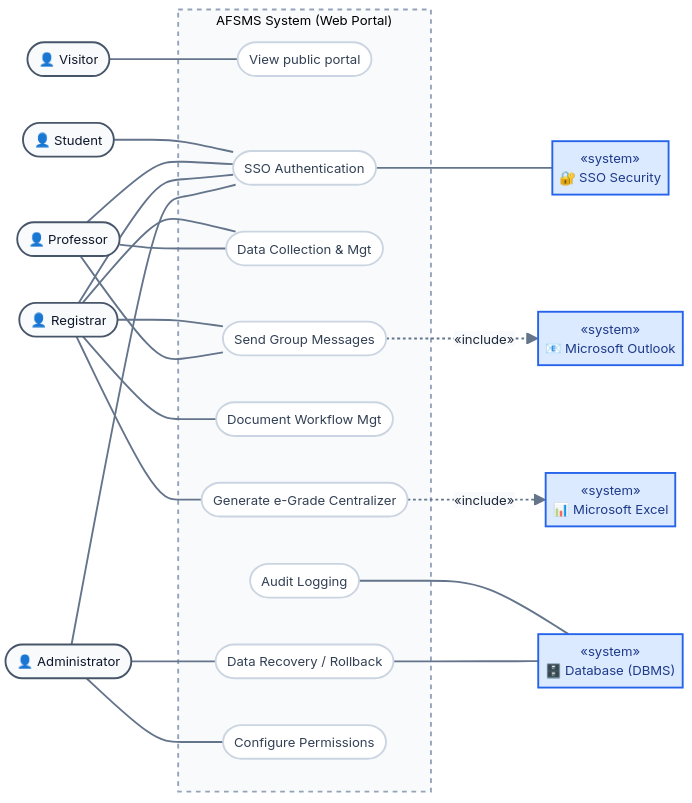
\includegraphics[width=0.85\textwidth]{1e.png}
      \vspace{0cm}
    }}
    \caption{System Use Case Diagram.}
    \label{fig:img1}
\end{figure}

\subsection{User Classes and Characteristics}
AFSMS serves the following user classes, ordered by importance to the system's core mission:

\begin{table}[H]
\centering
\small
\setlength{\arraystretch}{0.85}
\begin{tabularx}{\textwidth}{>{\raggedright\arraybackslash}p{2.2cm} >{\raggedright\arraybackslash}X >{\raggedright\arraybackslash}X >{\raggedright\arraybackslash}X}
\toprule
\textbf{User Class} & \textbf{Characteristics} & \textbf{Frequency of Use} & \textbf{Impact on Requirements} \\
\midrule
Registrar / Secretariat Staff (Primary) & Administrative professionals with intermediate computer skills. Proficient in MS Excel and Outlook but not IT experts. & Daily and continuous --- the heaviest system users. & Drive the need for optimized, error-proof interfaces (dropdowns), the ``3-minute'' usability requirement, and seamless Excel/Outlook integration. \\
\midrule
Professors / Teaching Staff & Professionals with varying technical expertise (novice to expert). & Intermittent, peaking at semester end and exam sessions. & Grade-entry interfaces must be intuitive with zero retraining needed. Access to student records requires SSO and role-based security. \\
\midrule
Students & Digitally literate users accustomed to responsive web apps; often use mobile devices. & Frequent during the academic year for schedules and grades. & Require read-only access limited to their own records. The portal must be platform-agnostic and fully responsive. \\
\midrule
System Administrators & IT professionals with advanced technical and database skills. & Occasional --- system setup, maintenance, or emergency recovery. & Drive requirements for complete activity logs, permission management, and database rollback/point-in-time recovery. \\
\midrule
General Public (Visitors) & Unauthenticated users with unknown technical backgrounds. & Occasional. & Drive the need for a public portal perspective with zero authentication, showing curricula and timetables. \\
\midrule
Quality Assurance (QA) / Testers & Professionals skilled in software validation and test execution. & Intensive during development and pre-deployment; intermittent during updates. & Drive the need for verifiable, unambiguous requirements and a dedicated testing section covering reporting, recovery, and performance. \\
\bottomrule
\end{tabularx}
\normalsize
\setlength{\arraystretch}{1.3}
\end{table}

\subsection{Operating Environment}
AFSMS uses a client-server architecture and operates in the following environments:

\textbf{Server Environment}
\begin{itemize}
    \item \textbf{Hardware:} Physical servers in the university data center or virtualized/cloud infrastructure with scalable processing and storage.
    \item \textbf{Operating Systems:} Linux (Ubuntu Server 22.04/24.04 LTS, CentOS) or Windows Server (2019, 2022).
    \item \textbf{Software:} An RDBMS supporting complex queries, offline backups, and point-in-time recovery.
\end{itemize}

\textbf{Client Environment}
\begin{itemize}
    \item \textbf{Hardware:} Any internet-connected device --- desktop PCs, laptops, tablets, or smartphones.
    \item \textbf{Operating Systems:} Windows (10, 11), macOS, desktop Linux, Android, iOS.
    \item \textbf{Browsers:} Google Chrome 100+, Mozilla Firefox 100+, Microsoft Edge, Apple Safari.
\end{itemize}

\textbf{Compatibility}

On registrar workstations, the client must coexist with Microsoft Excel (2016, 2019, 2021, or Microsoft 365) and Microsoft Outlook without memory conflicts, supporting CSV/XLS import/export and institutional communication.

\subsection{Design and Implementation Constraints}
\begin{itemize}
    \item \textbf{Regulatory Policies:} The system must comply with EU/Romanian GDPR for personal student data and with the University of Craiova's academic data retention policies.
    \item \textbf{Hardware/Memory:} The server requires scalable storage for comprehensive activity logs needed by point-in-time recovery.
    \item \textbf{Technologies:} The backend must use an RDBMS. The frontend must use standard web technologies (HTML/CSS/JS) for cross-platform compatibility with no local client installation.
    \item \textbf{Security and Protocols:} All data transfers must use HTTPS. Authentication must support institutional SSO.
    \item \textbf{Application Interfaces:} Export and communication modules must interface with Microsoft Excel (.XLS/.CSV) and Microsoft Outlook.
    \item \textbf{Design Conventions:} Developers must use selection lists (dropdowns) over free-text fields for standardized data entry. Reports must display in tabular format.
    \item \textbf{Audit and Concurrency:} The DBMS must support full activity logging (audit) and point-in-time rollback. The system must handle concurrent access during peak exam sessions without data corruption.
\end{itemize}

\subsection{User Documentation}
The following documentation, organized by user role, will accompany AFSMS.

\subsubsection{Delivered Documentation Components}
\begin{itemize}
    \item \textbf{Registrar \& Secretariat Staff Operations Manual:}
    \begin{itemize}
        \item \textit{Scope:} Complete guide for daily workflows and data entry.
        \item \textit{Contents:} Step-by-step instructions for dropdown-based data collection, electronic document circulation, advanced search filters, Excel import/export, Outlook communications, and generating the e-Transcript and e-Grade Centralizer.
    \end{itemize}
    \item \textbf{Professors \& Teaching Staff Quick Start Guide:}
    \begin{itemize}
        \item \textit{Scope:} Concise, visual tutorial for faculty-relevant features.
        \item \textit{Contents:} SSO authentication, locating study formations, entering session grades, and finalizing evaluation records.
    \end{itemize}
    \item \textbf{System \& Database Administrator Guide:}
    \begin{itemize}
        \item \textit{Scope:} Technical documentation for IT staff.
        \item \textit{Contents:} Site adaptation procedures (curricula, grid values), user privilege mapping, DBMS management, activity log interpretation, offline backups, and point-in-time recovery (rollback).
    \end{itemize}
    \item \textbf{Student Portal Guide (Online Help):}
    \begin{itemize}
        \item \textit{Scope:} Brief FAQ embedded in the private portal.
        \item \textit{Contents:} Viewing personal schedules, interpreting grades, and requesting administrative documents.
    \end{itemize}
\end{itemize}

\subsubsection{Interactive and In-App Documentation}
\begin{itemize}
    \item \textbf{Context-Sensitive Help:} Embedded tooltips next to complex fields and dropdowns.
    \item \textbf{Error Resolution Prompts:} Client-side validation errors include resolution suggestions (e.g., ``Invalid format: Ensure the Excel file matches the provided .XLS template before importing'').
\end{itemize}

\subsubsection{Delivery Formats and Tooling}
\begin{itemize}
    \item \textbf{Web-Based Documentation:} Online help section integrated within the web portal (guides, FAQs, contextual help).
    \item \textbf{PDF Manuals:} Registrar, Professor, and Administrator guides in PDF for offline access and archiving.
\end{itemize}
All documentation will be updated alongside major software releases.

\subsubsection{Documentation Standards and Compliance}
\begin{itemize}
    \item \textbf{ISO/IEC/IEEE 26514:2022:} Standard for user documentation design and development.
    \item \textbf{WCAG 2.2 (Level AA):} HTML5 and PDF documentation must meet accessibility requirements (screen reader compatibility, color contrast, keyboard navigation).
    \item \textbf{GDPR Compliance:} All sample data and screenshots must use anonymized, synthetic data --- no real student PII.
\end{itemize}

\subsection{Assumptions and Dependencies}
The following assumed factors and external dependencies influence the requirements in this SRS. If any prove false, the affected requirements will need revision.

\subsubsection{Assumptions (Factors Assumed to be True)}

\textbf{Infrastructure and Provisioning:}
\begin{itemize}
    \item \textit{Assumed:} The university IT department will provide a data center or cloud-hosting environment with adequate availability during academic periods and sufficient bandwidth for exam-season traffic.
    \item \textit{If false:} The SRS must add requirements for an external cloud architecture (e.g., AWS/Azure) and load-balancing.
\end{itemize}

\textbf{Centralized SSO Availability:}
\begin{itemize}
    \item \textit{Assumed:} The university SSO subsystem provides a stable authentication endpoint (SAML 2.0 or OAuth 2.0).
    \item \textit{If false:} The SRS must add requirements for secure password hashing, credential storage, account recovery, and MFA.
\end{itemize}

\textbf{Browser Standards and Connectivity:}
\begin{itemize}
    \item \textit{Assumed:} All users have reliable internet and devices capable of rendering HTML5 and ES6 JavaScript.
    \item \textit{If false:} The SRS must add requirements for offline synchronization and legacy browser polyfills.
\end{itemize}

\textbf{Open-Source / Commercial Libraries:}
\begin{itemize}
    \item \textit{Assumed:} The team has unrestricted access to libraries for generating CSV, XML, XLS, and PDF exports.
    \item \textit{If false:} Export requirements must be scaled down, or the budget/timeline expanded.
\end{itemize}

\textbf{Administrative User Training:}
\begin{itemize}
    \item \textit{Assumed:} Registrar staff will complete a mandatory 1-hour training session before deployment.
    \item \textit{If false:} The 3-minute usability benchmark cannot be fairly evaluated at UAT and must be removed.
\end{itemize}

\subsubsection{Dependencies (External Factors Relied Upon)}

\textbf{Microsoft Office Ecosystem:}

The export, import, and communication modules depend on Microsoft Excel and Microsoft Outlook being available and licensed on registrar machines. If Microsoft deprecates interoperability protocols or changes .XLS parsing rules, integration modules will need refactoring.

\textbf{Legacy Data Availability (Site Adaptation):}

Launch depends on the secretariat providing cleansed, structured legacy data (historical records, curricula, past grid values) for database seeding. Delays or formatting errors in this data will block deployment.

\textbf{Regulatory Environment:}

Logging, data retention, and rollback features depend on current EU/Romanian GDPR legislation and Romanian Ministry of Education archiving mandates. Legislative changes will force revisions to database architecture and data-pruning logic.

\textbf{Institutional Network Security:}

Automated notifications and user authentication depend on the university IT department whitelisting the application servers for outbound SMTP traffic and inbound SSO callbacks.


% --- SECTION 3: EXTERNAL INTERFACE REQUIREMENTS ---
\section{External Interface Requirements}

\subsection{User Interfaces}
AFSMS provides a web-based GUI accessible through modern browsers, organized into:
\begin{itemize}
    \item \textbf{Public Portal:} Unauthenticated, read-only access.
    \item \textbf{Private Portal:} Authenticated via university SSO with role-based access control (registrar staff, professors, students, administrators).
\end{itemize}

\subsubsection{Logical Characteristics and Screen Organization}
\begin{itemize}
    \item \textbf{Layout:} A persistent two-pane design --- a fixed, role-based navigation sidebar on the left and a dynamic workspace on the right. Breadcrumb navigation appears at the top of the workspace.
    \item \textbf{Screen Formats:} All academic records (grade registers, centralizers) use a standard tabular format mirroring MS Excel for familiarity.
    \item \textbf{Standardized Elements:} Every authenticated screen includes a persistent top header with a universal search bar, user profile/logout controls, and a ``Help'' icon for context-sensitive assistance.
    \item \textbf{Keyboard Shortcuts:} The system supports grid-navigation shortcuts (Tab to cycle columns, Enter to save the row and advance) to optimize repetitive data entry.
\end{itemize}

\subsubsection{UI Optimization and Verifiable Usability}
\begin{itemize}
    \item \textbf{Selection-Only Mandate:} The UI must use searchable dropdown menus (e.g., Select2/React-Select) for all relational data inputs (study formations, subjects, academic years). Free-text fields are allowed only when strictly required for non-standardized descriptions.
    \item \textbf{Error Message Standards:} Brief, non-technical error messages appear adjacent to the offending input field (e.g., ``Grade must be an integer between 1 and 10''). System-level errors include a ``More Info'' toggle for technical details.
    \item \textbf{Verifiable Usability Requirement:} A secretariat staff member shall compile and export a complete semester e-Grade Centralizer for a 30-student group in under 3 minutes, after no more than 1 hour of basic training.
\end{itemize}

\begin{figure}[htbp]
    \centering
    \begin{minipage}{0.49\textwidth}
        \centering
        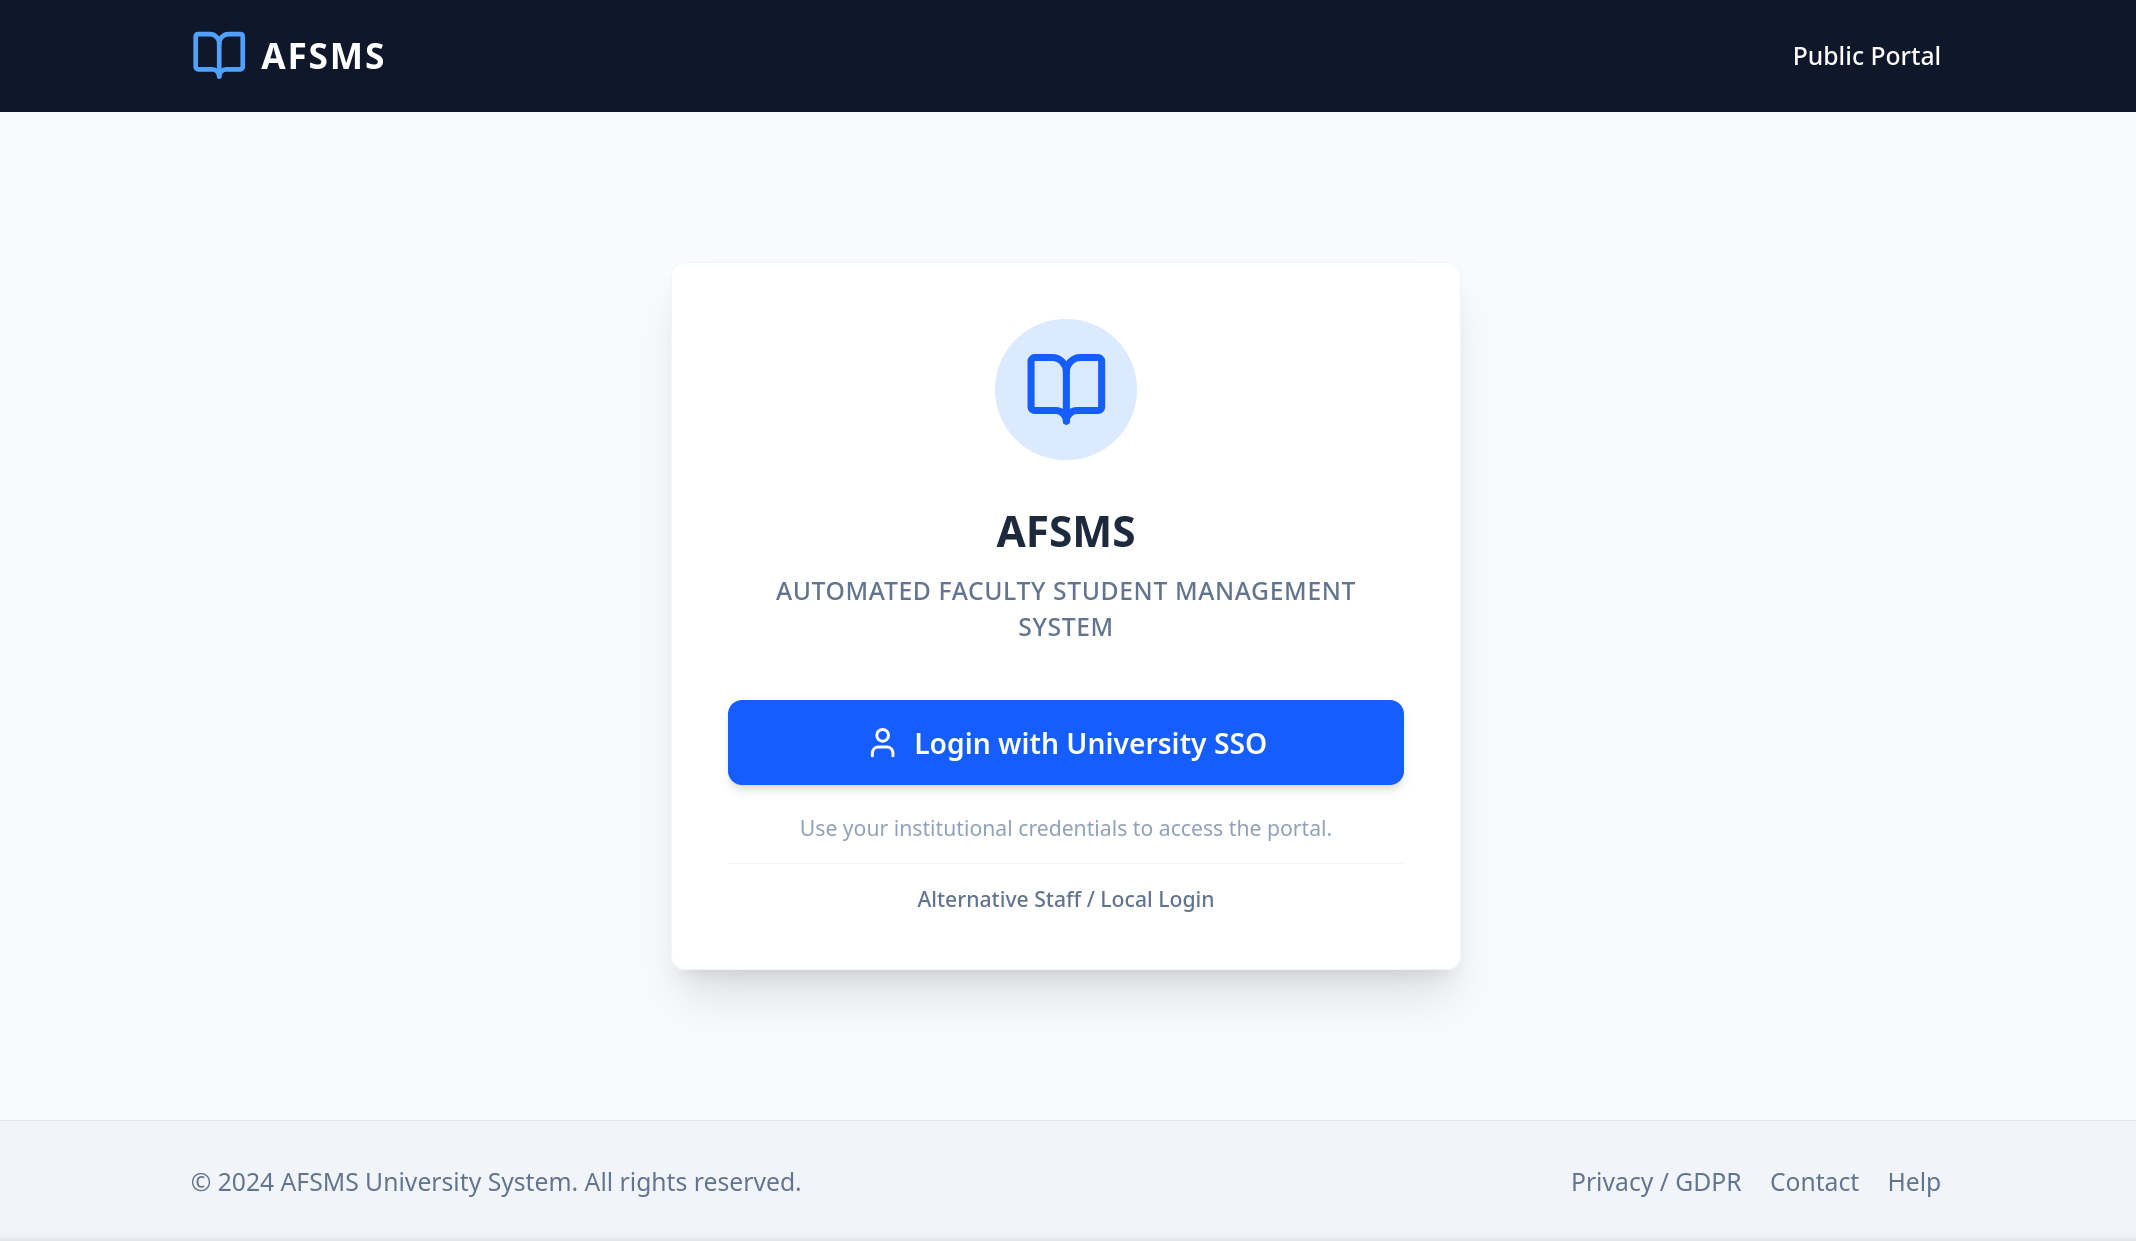
\includegraphics[width=\textwidth]{6.png}
        \caption{Students \& Curricula Management UI.}
        \label{fig:img6}
    \end{minipage}
    \hfill
    \begin{minipage}{0.49\textwidth}
        \centering
        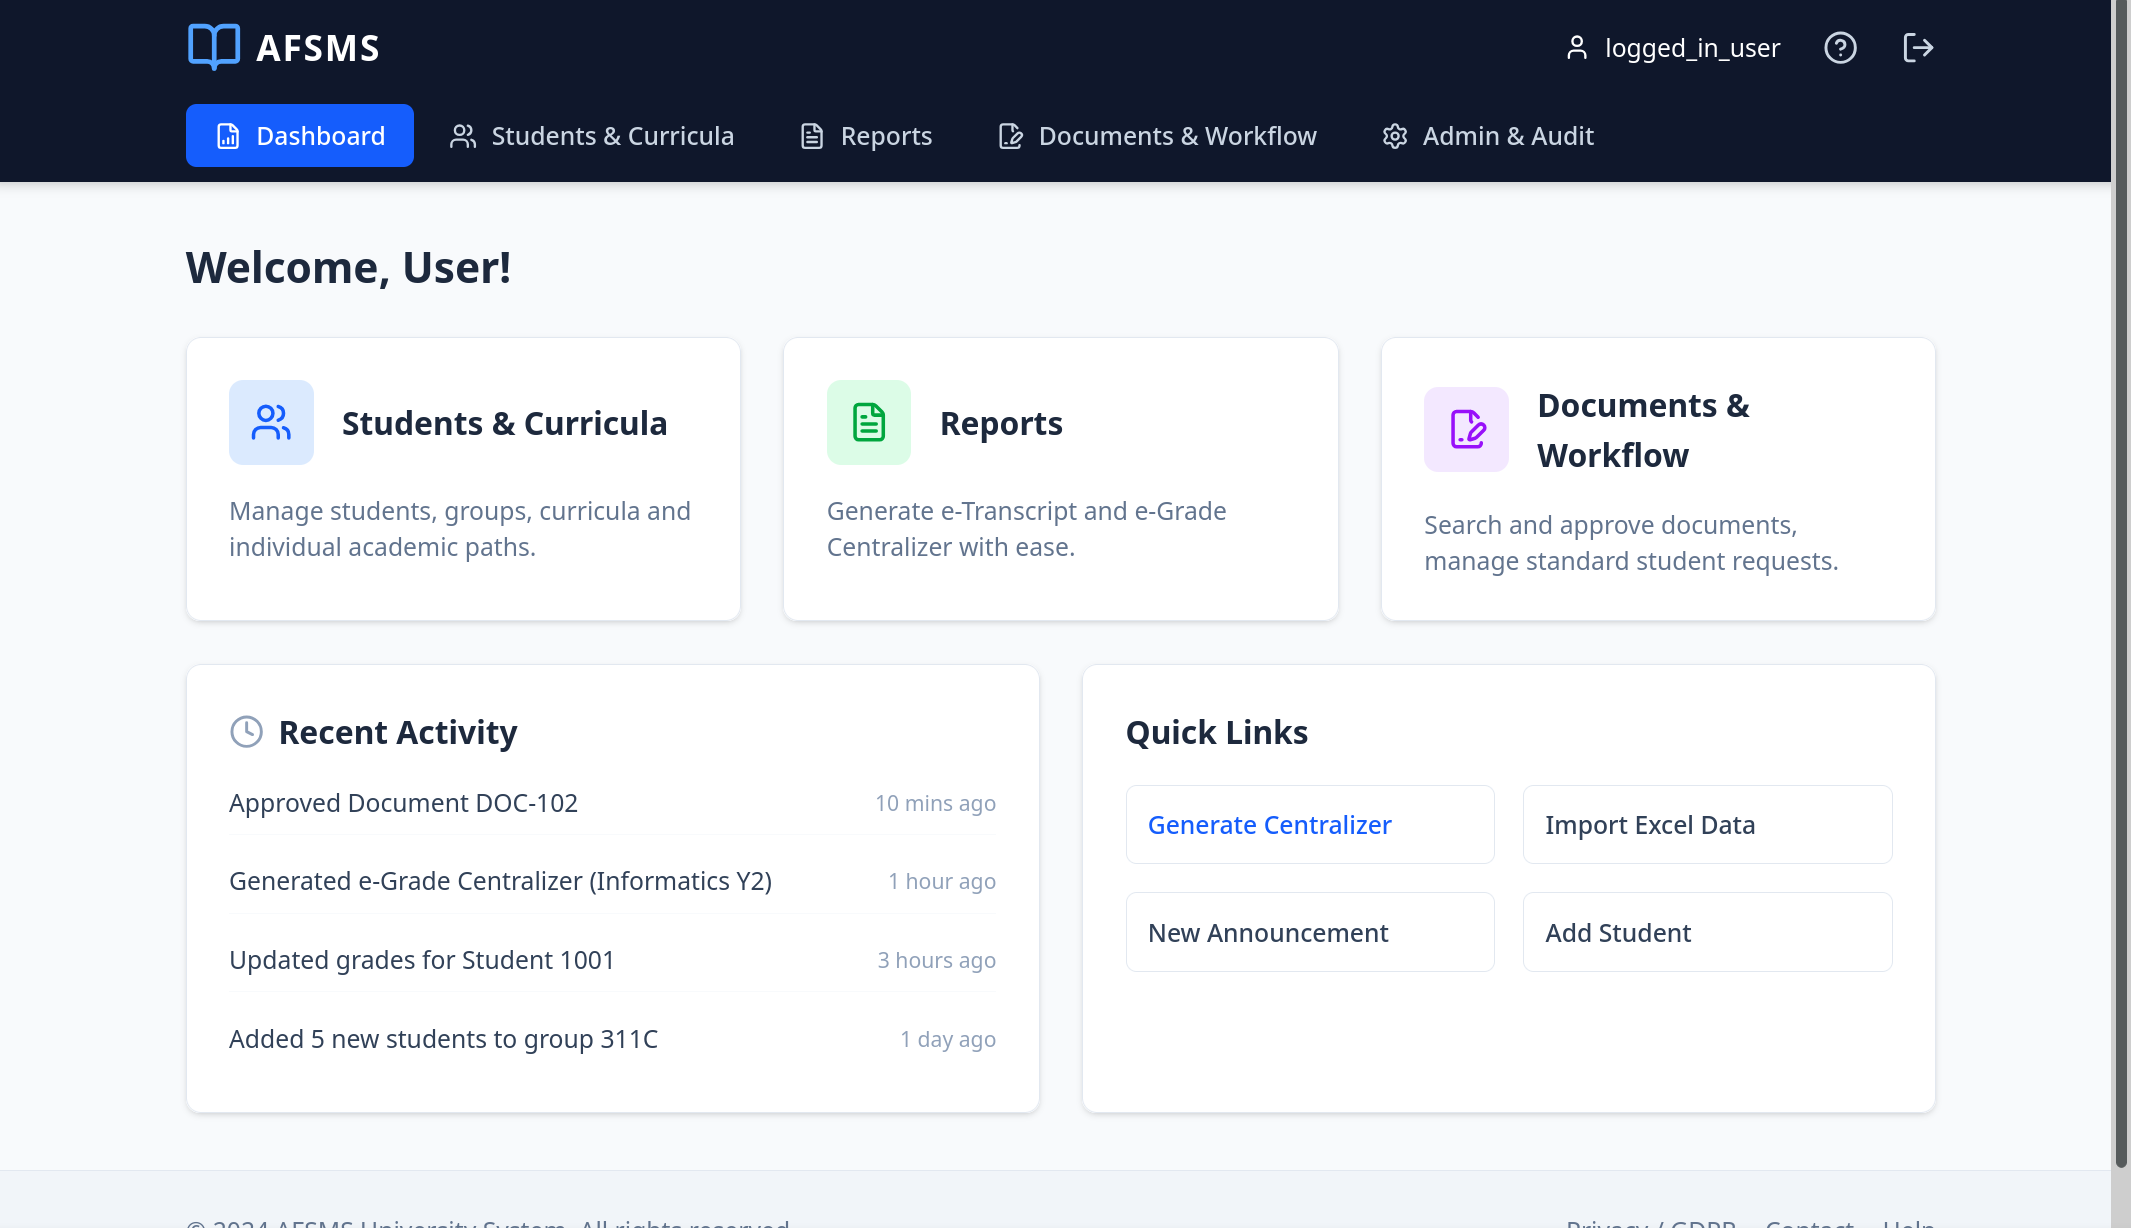
\includegraphics[width=\textwidth]{7.png}
        \caption{Data Collection Flowchart.}
        \label{fig:img7}
    \end{minipage}
\end{figure}

\begin{figure}[htbp]
    \centering
    \begin{minipage}{0.49\textwidth}
        \centering
        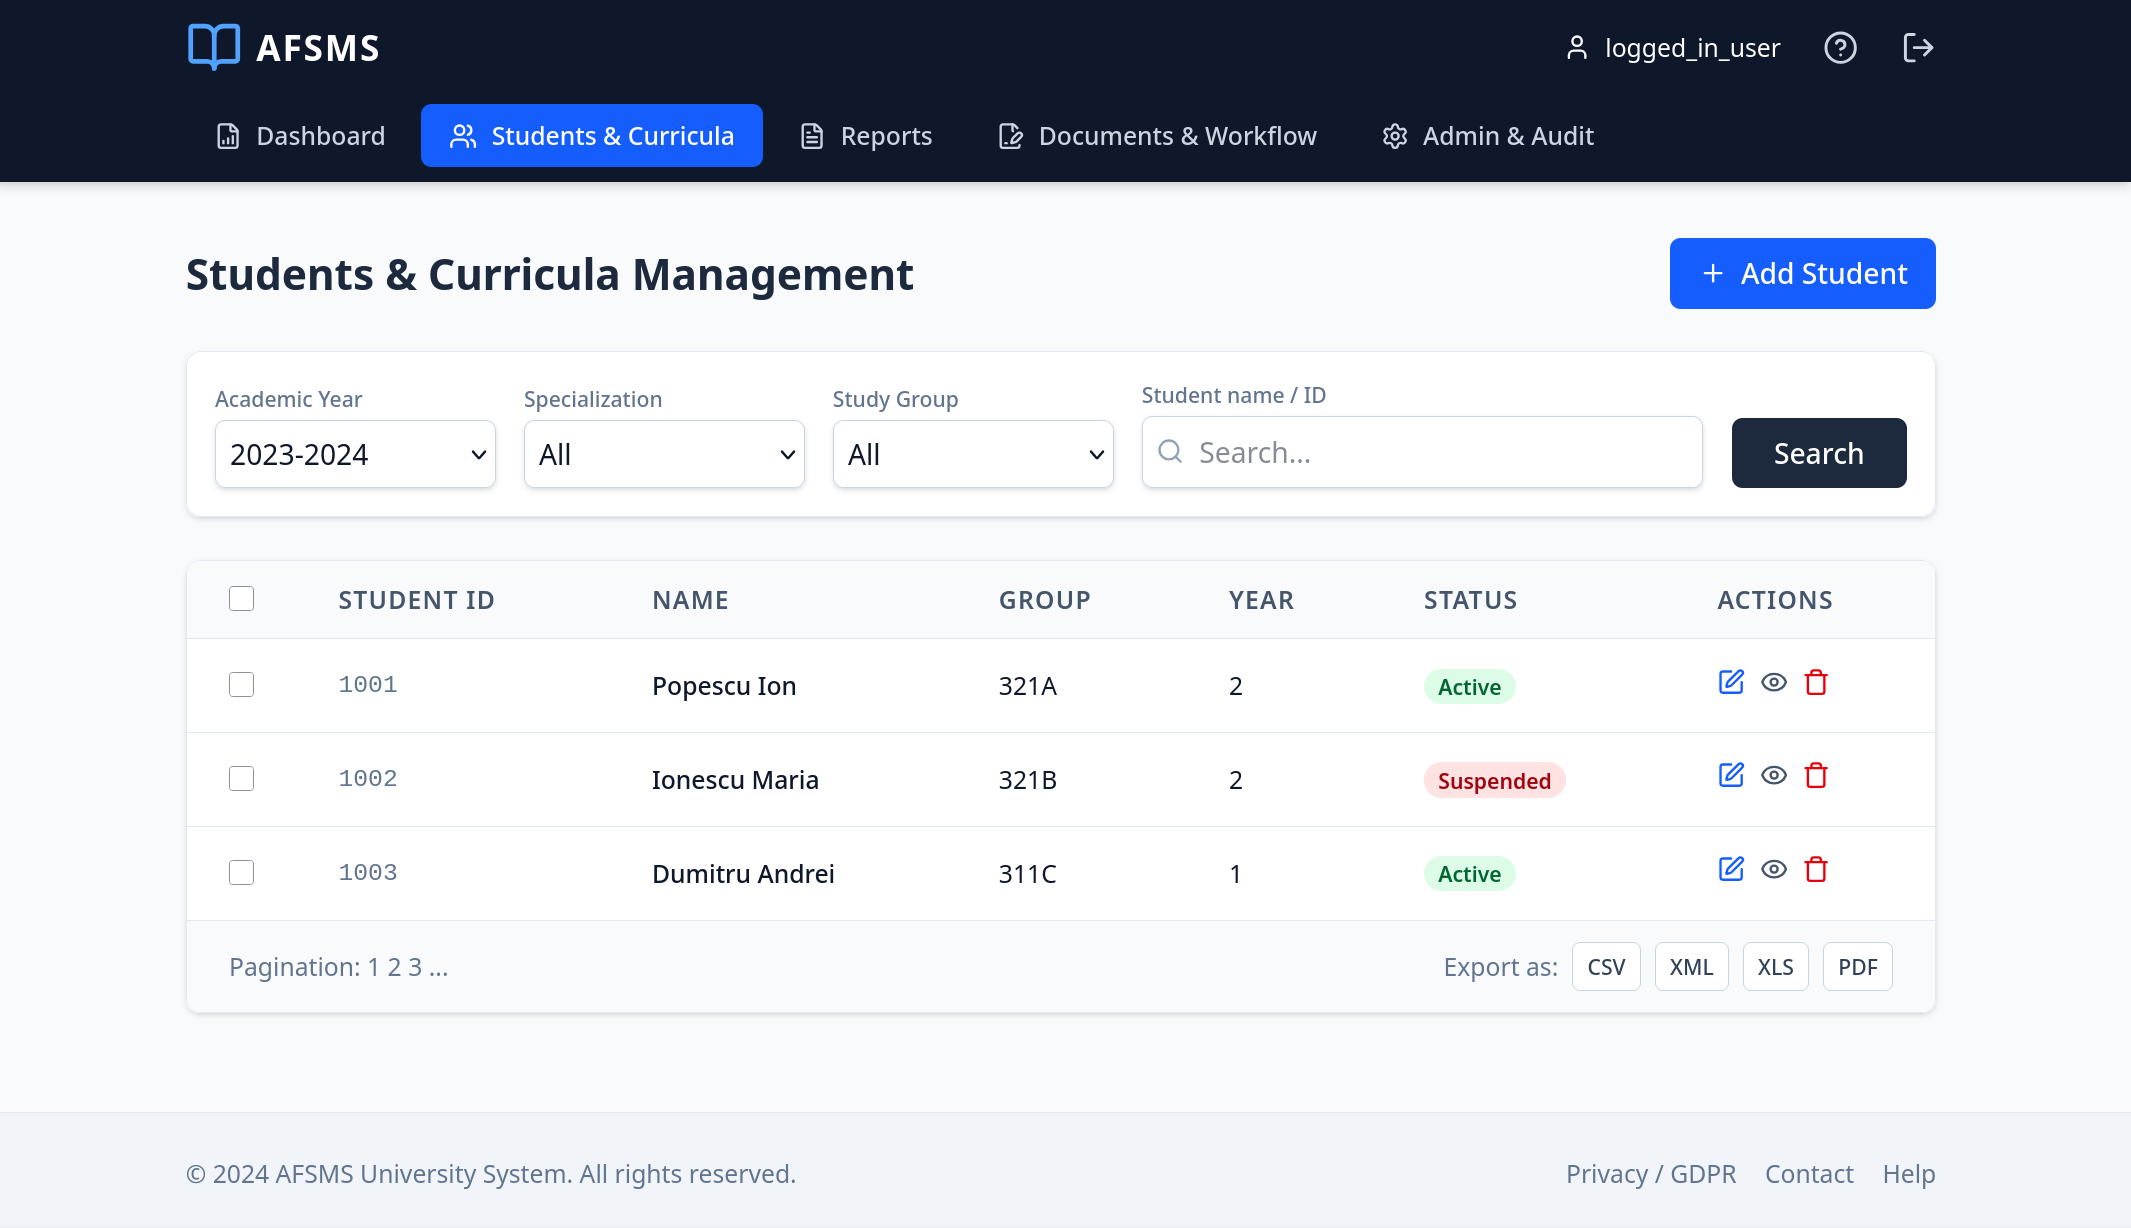
\includegraphics[width=\textwidth]{8.png}
        \caption{Reports - e-Grade Centralizer UI.}
        \label{fig:img8}
    \end{minipage}
    \hfill
    \begin{minipage}{0.49\textwidth}
        \centering
        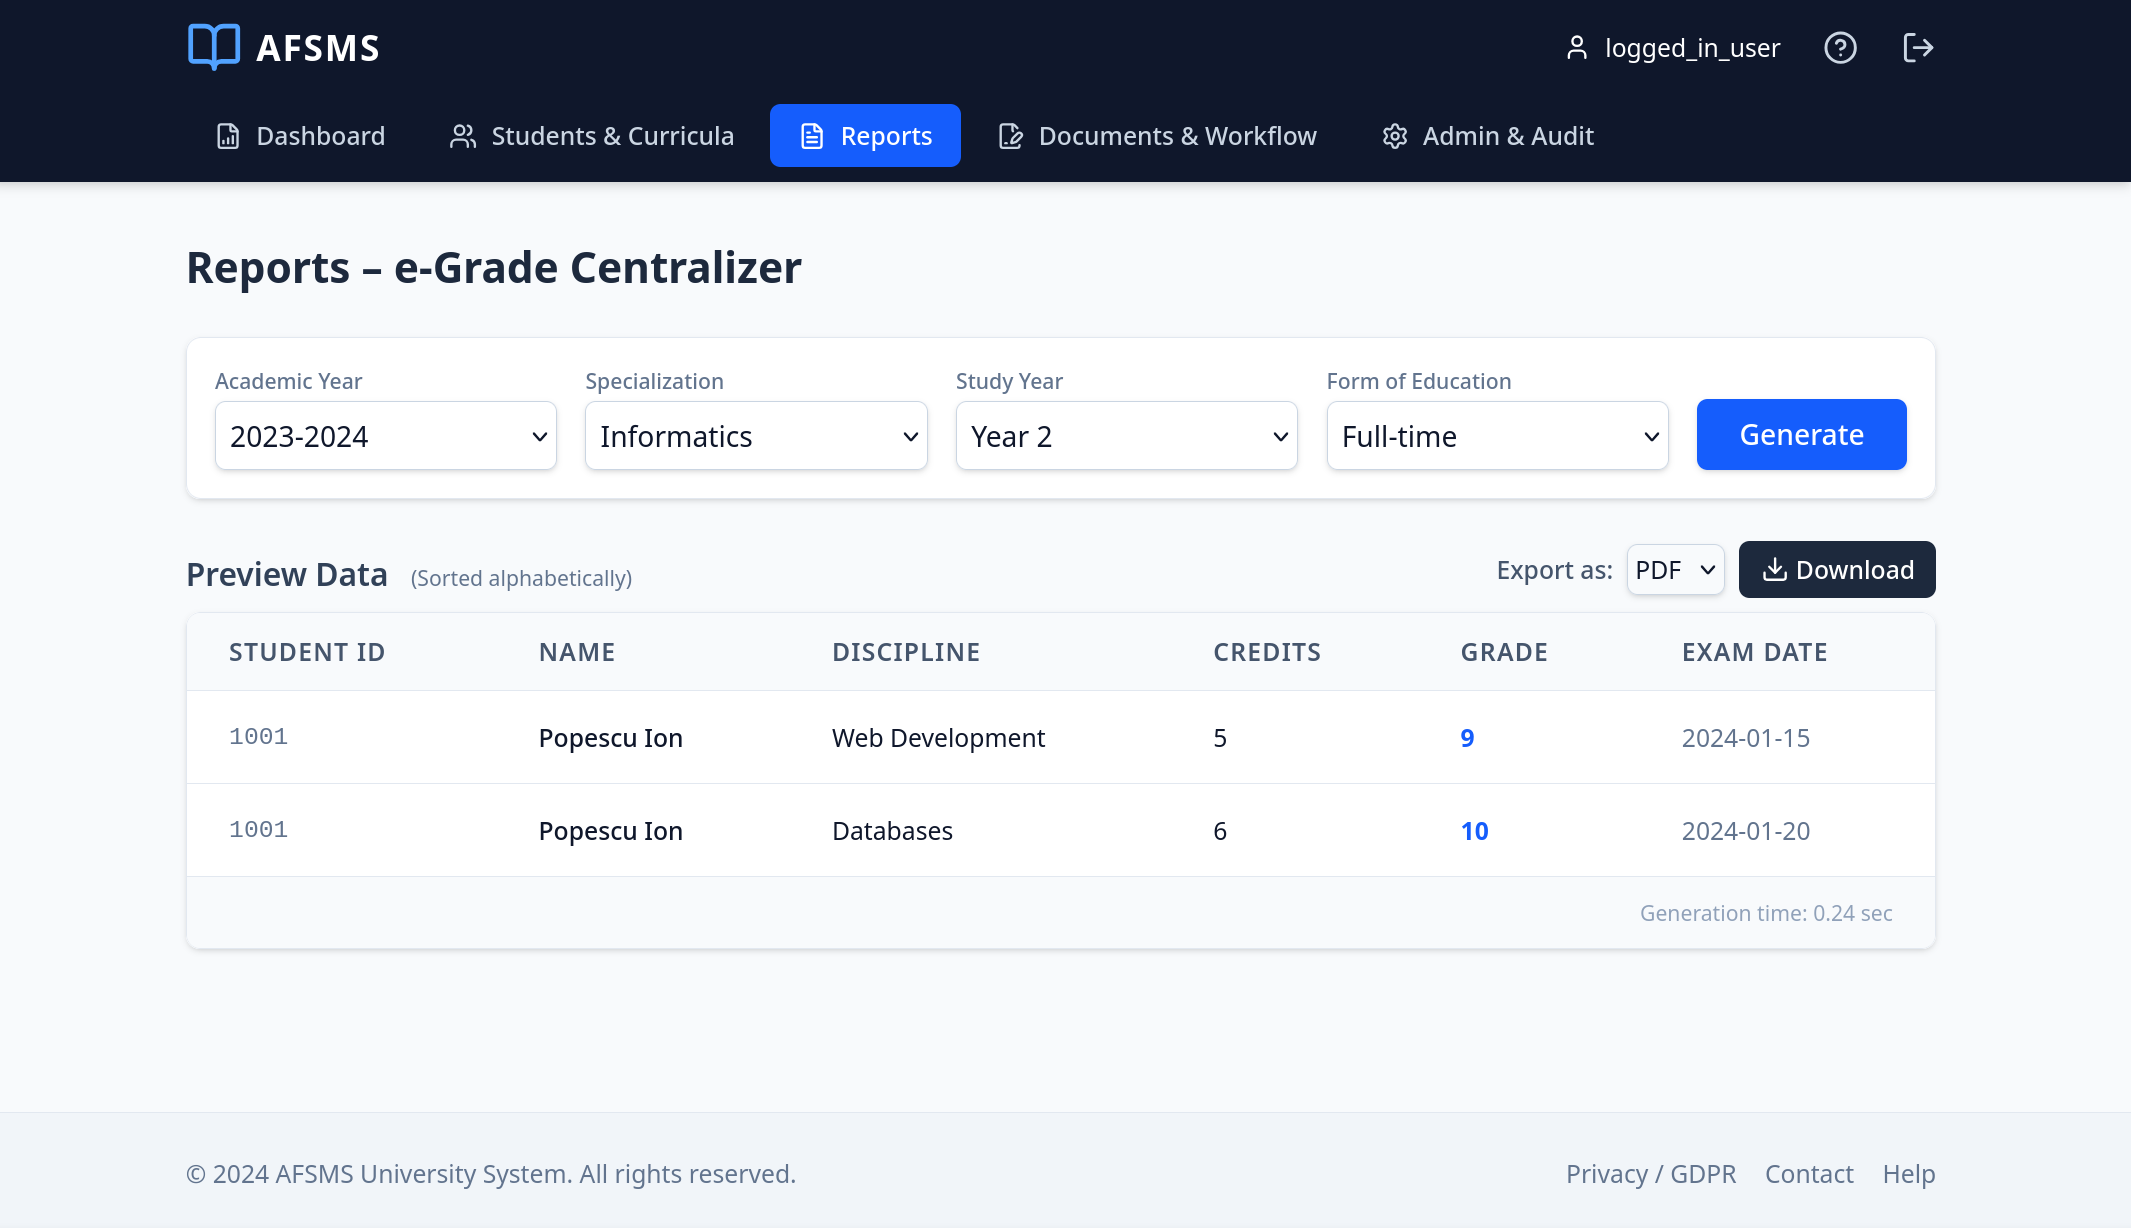
\includegraphics[width=\textwidth]{9.png}
        \caption{Documents \& Workflow UI.}
        \label{fig:img9}
    \end{minipage}
\end{figure}

\begin{figure}[htbp]
    \centering
    \begin{minipage}{0.49\textwidth}
        \centering
        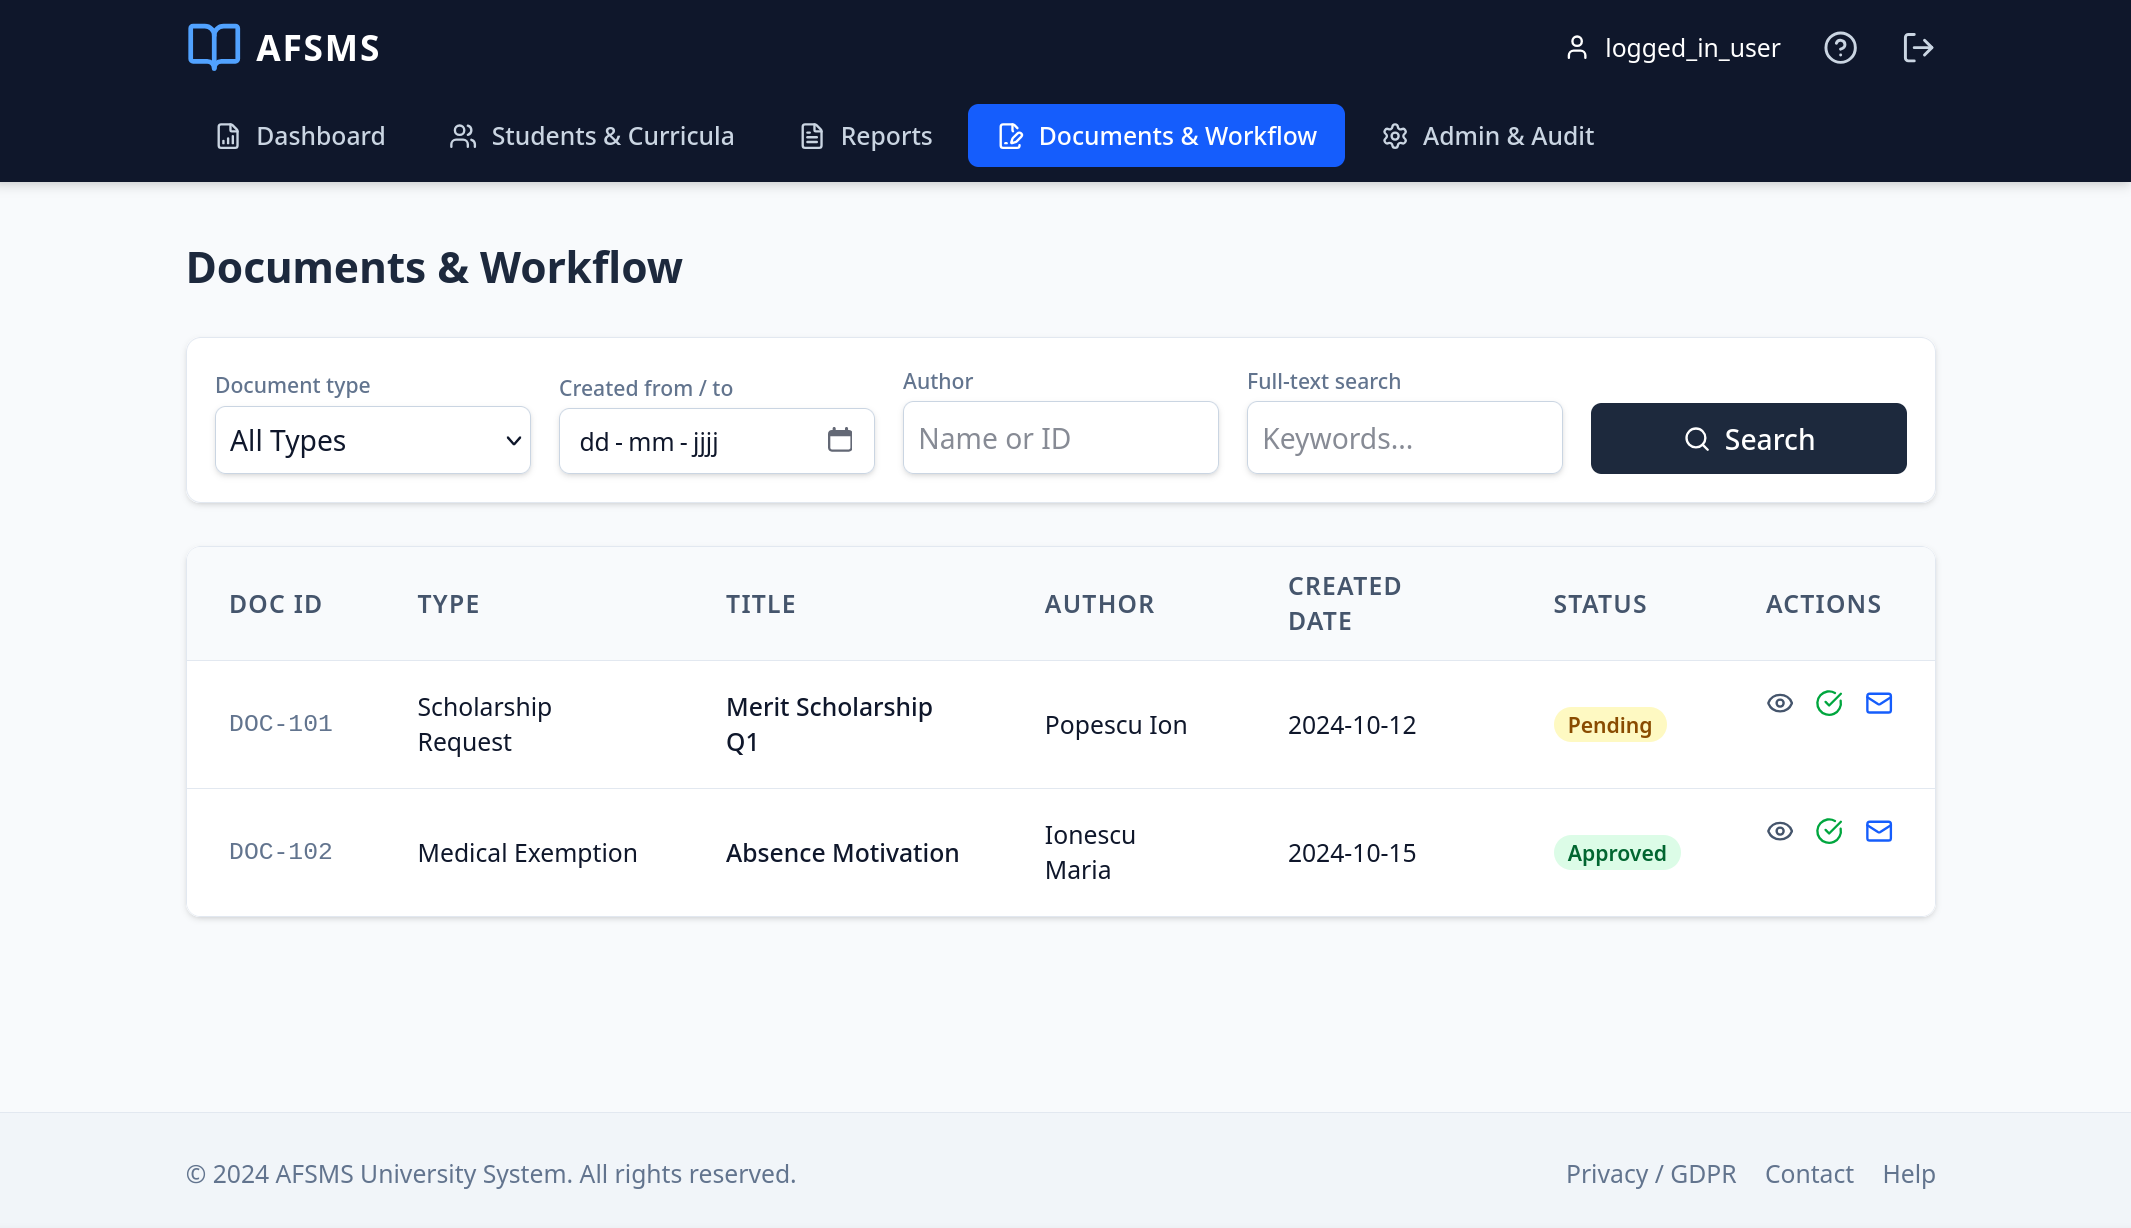
\includegraphics[width=\textwidth]{10.png}
        \caption{User Groups \& Messaging.}
        \label{fig:img10}
    \end{minipage}
    \hfill
    \begin{minipage}{0.49\textwidth}
        \centering
        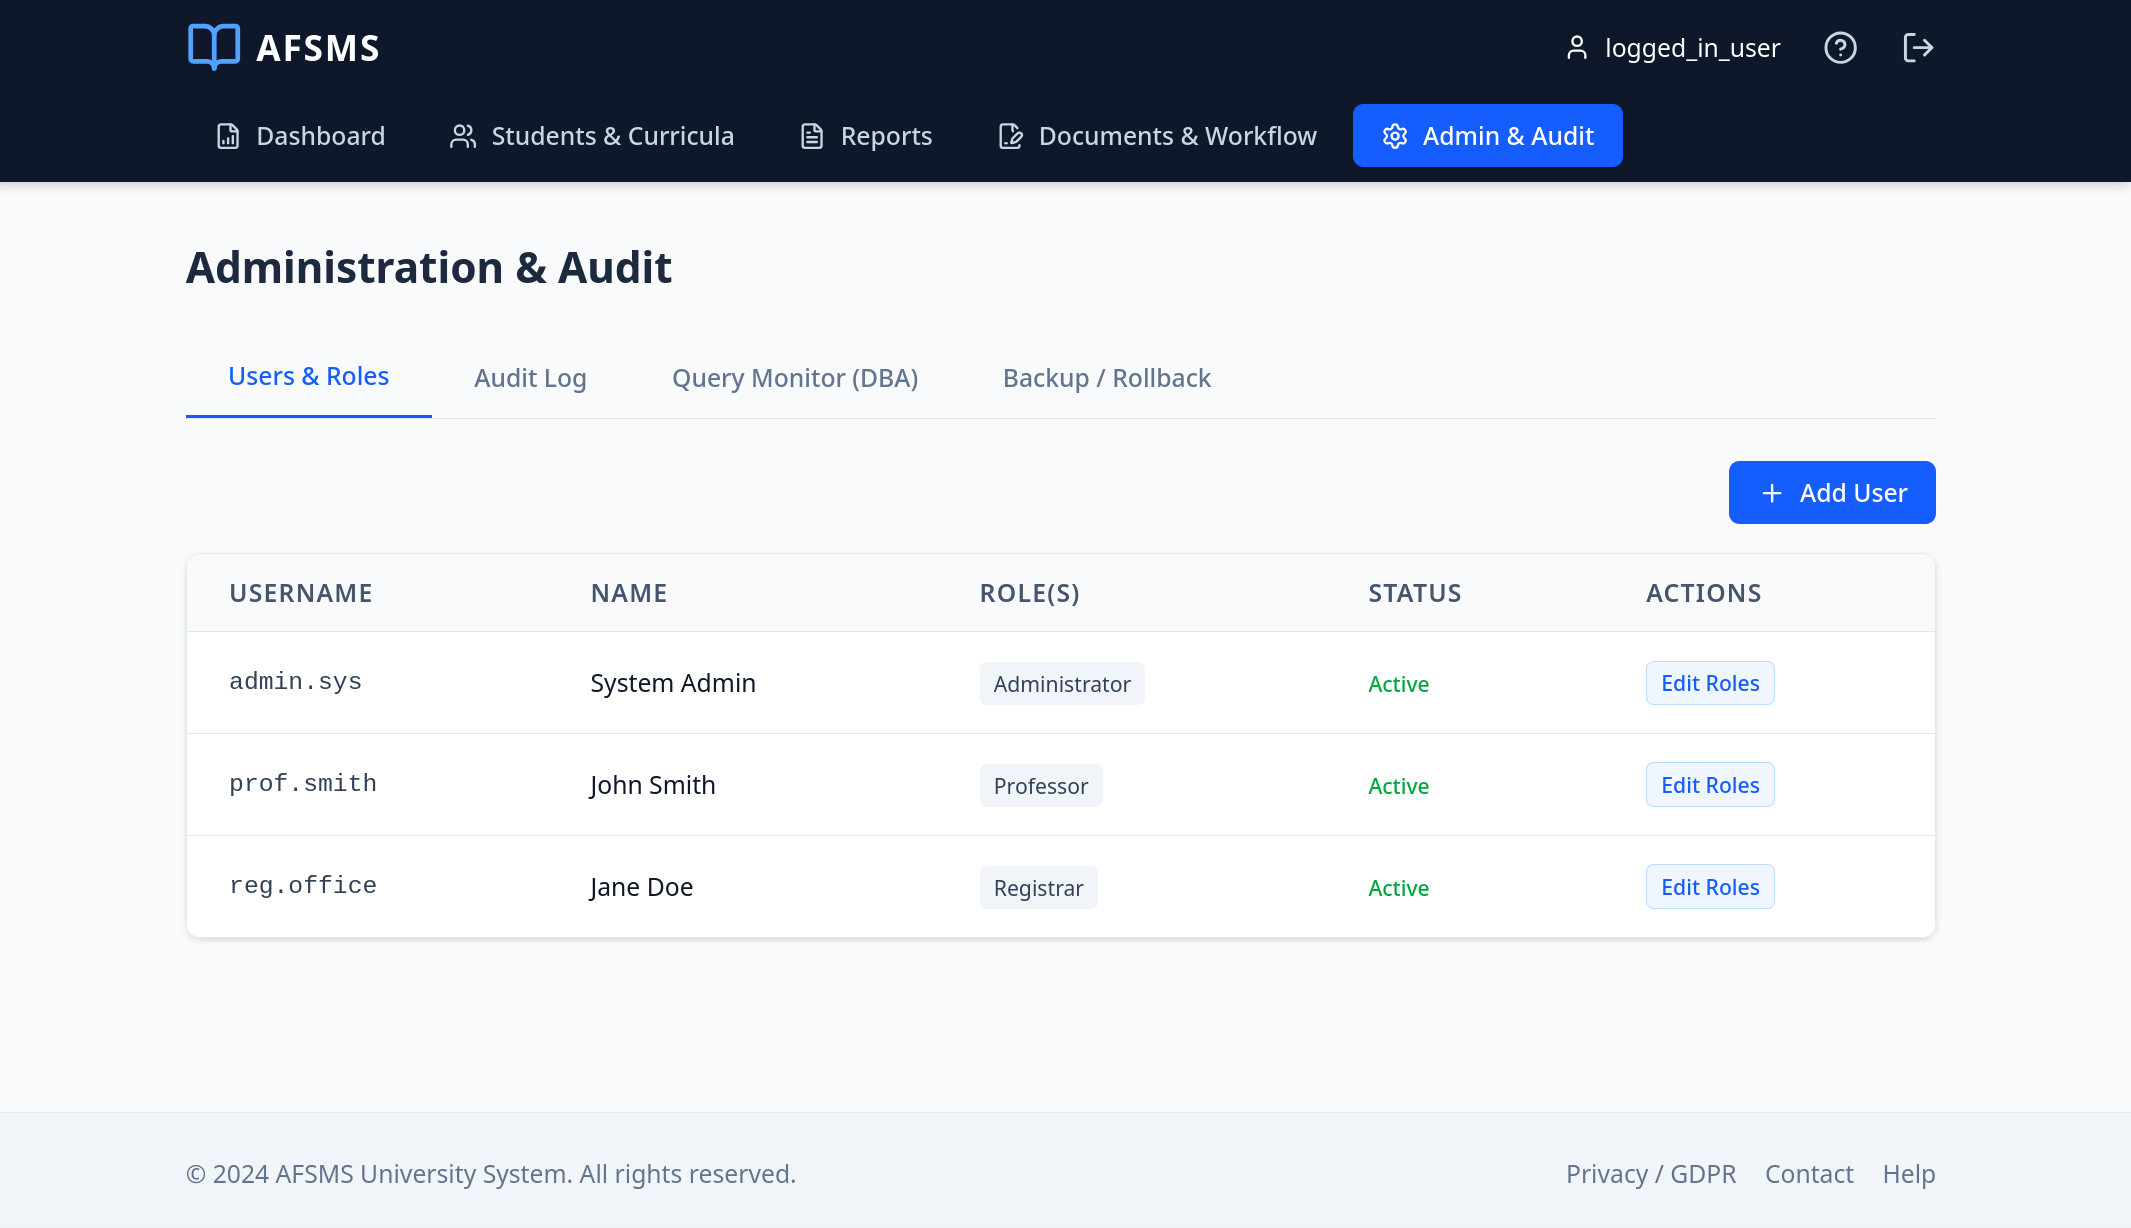
\includegraphics[width=\textwidth]{11.png}
        \caption{Administration \& Audit - Users \& Roles.}
        \label{fig:img11}
    \end{minipage}
\end{figure}

\begin{figure}[htbp]
    \centering
    \begin{minipage}{0.49\textwidth}
        \centering
        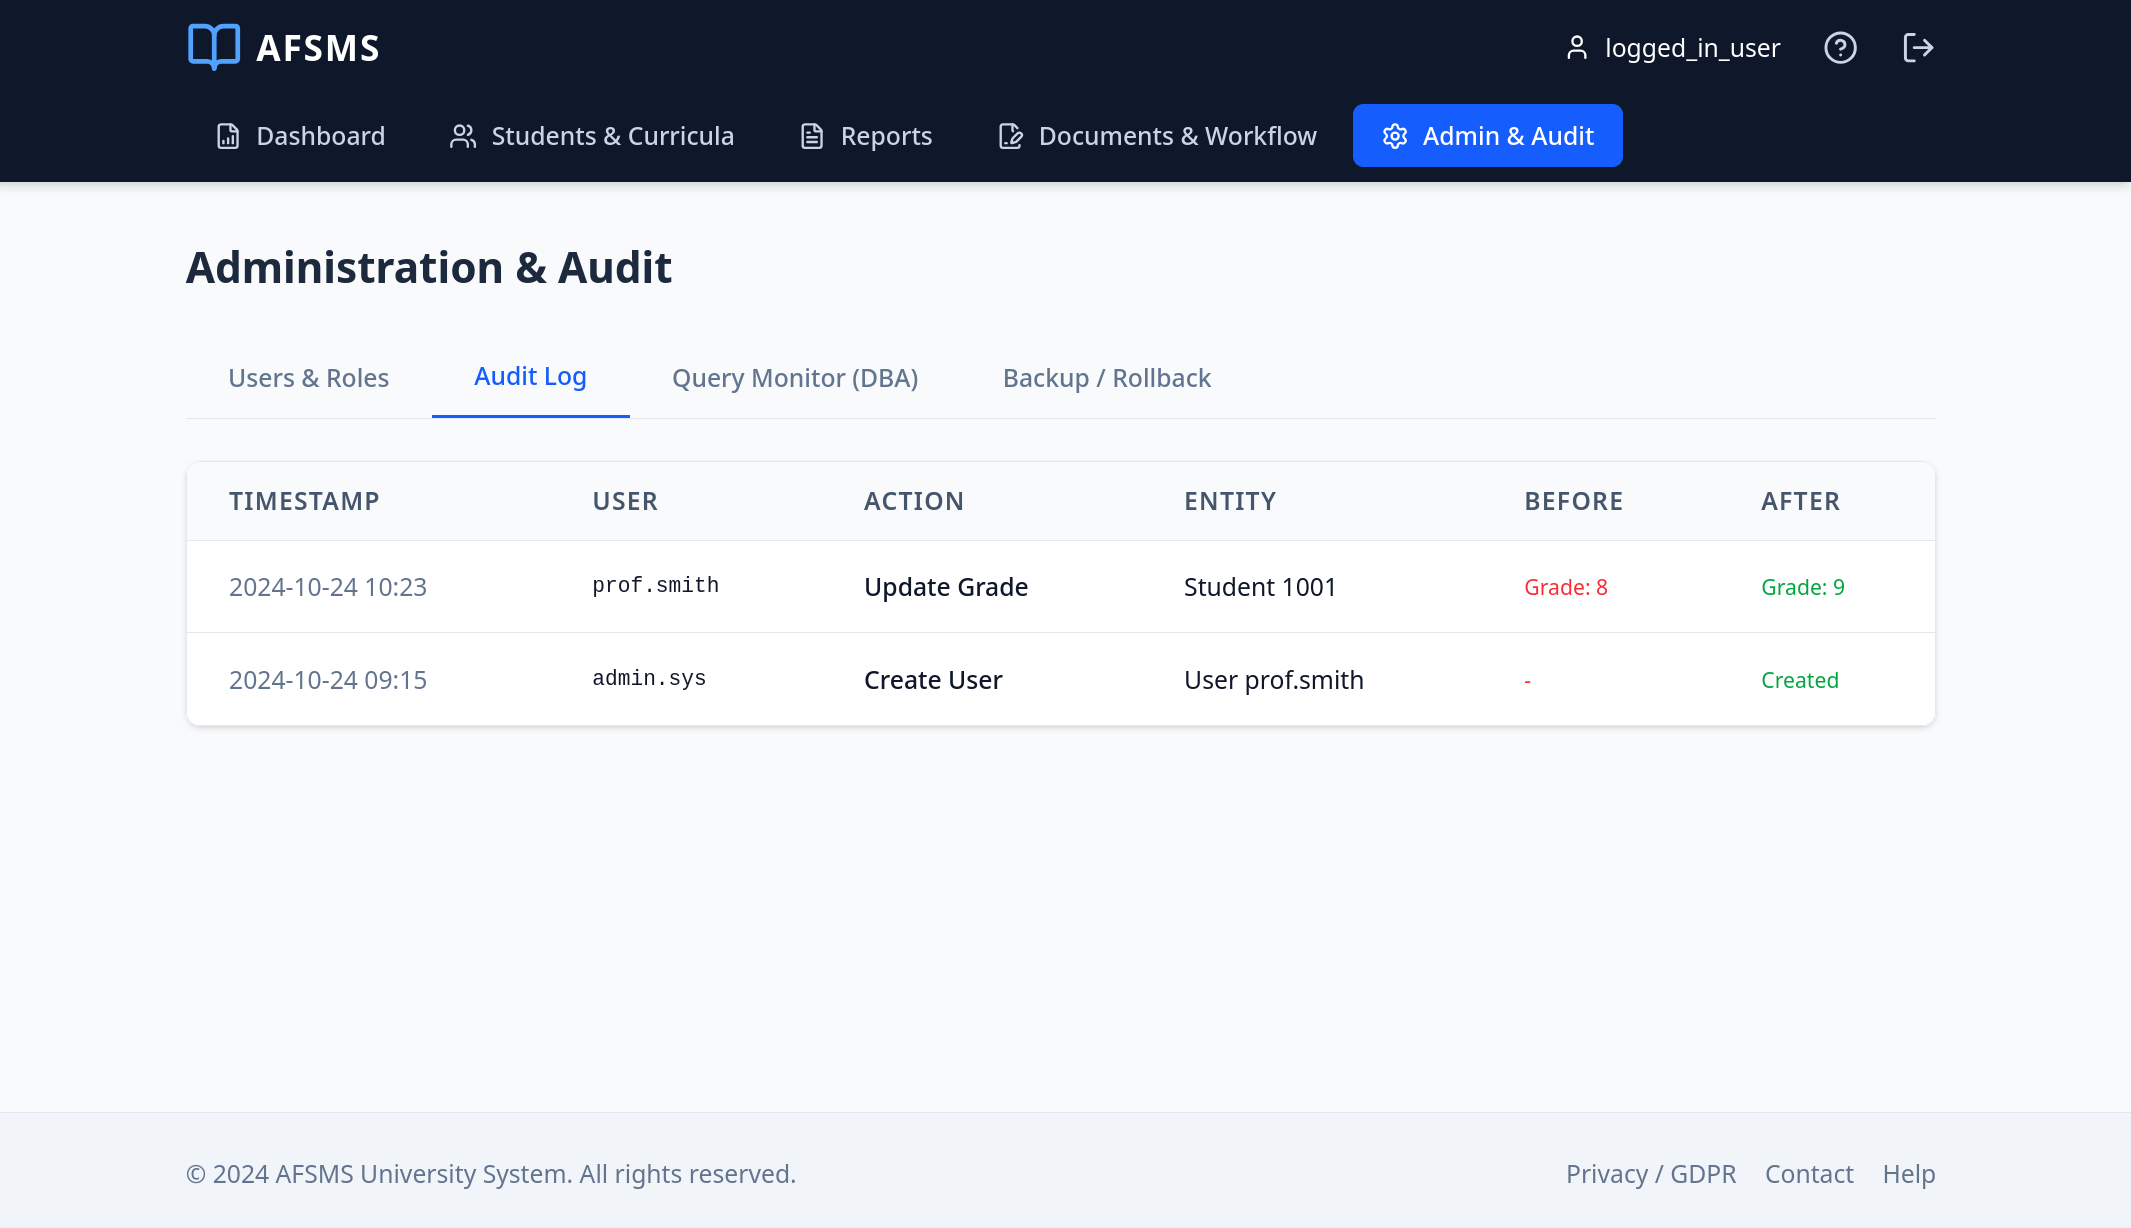
\includegraphics[width=\textwidth]{12.png}
        \caption{Administration \& Audit - Audit Log.}
        \label{fig:img12}
    \end{minipage}
    \hfill
    \begin{minipage}{0.49\textwidth}
        \centering
        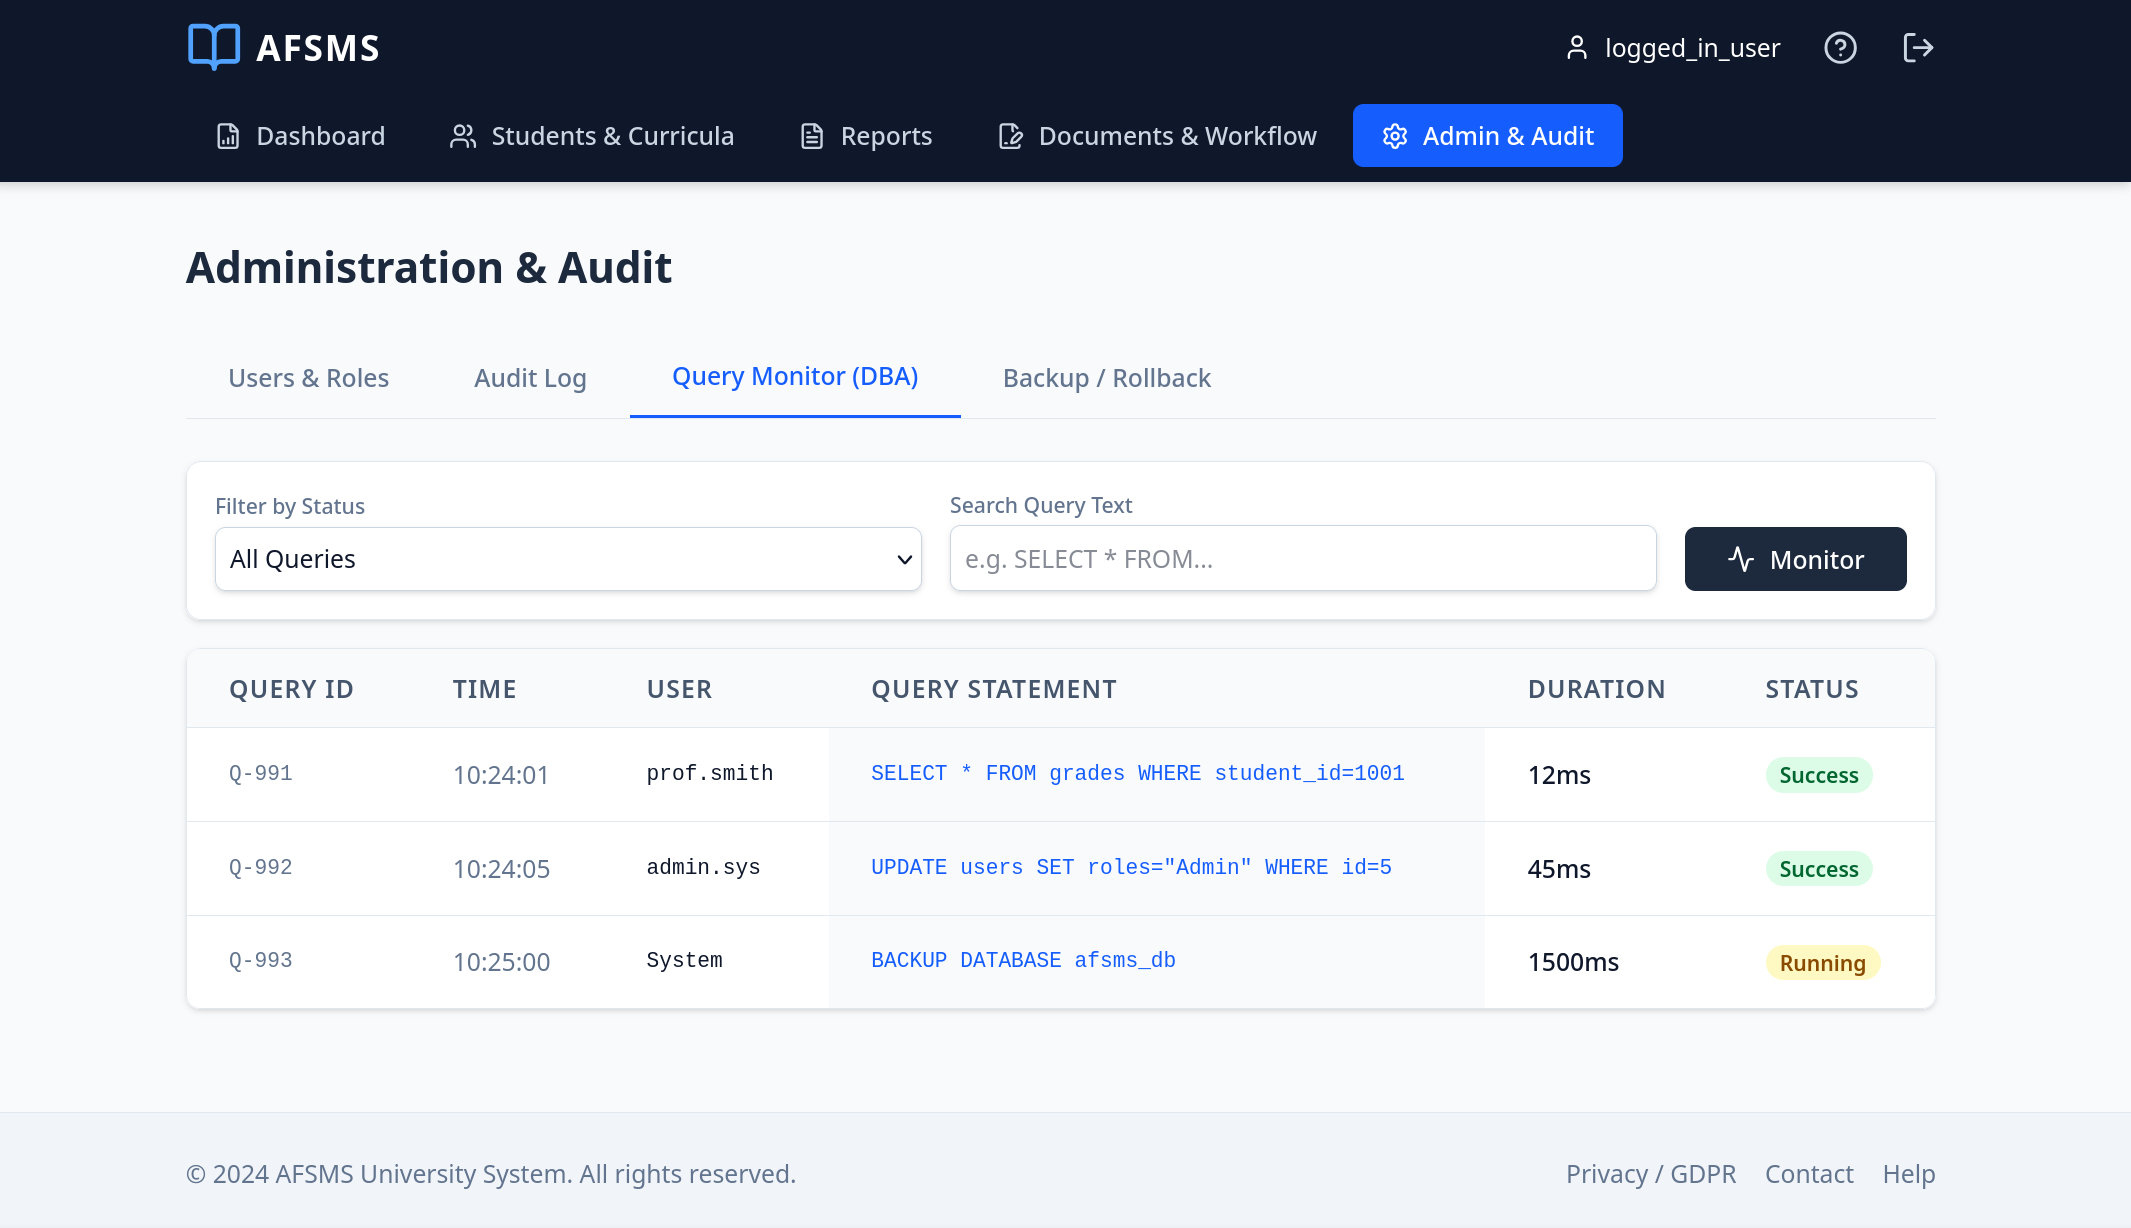
\includegraphics[width=\textwidth]{13.png}
        \caption{Administration \& Audit - Backup / Rollback.}
        \label{fig:img13}
    \end{minipage}
\end{figure}

\begin{figure}[htbp]
    \centering
    \begin{minipage}{0.49\textwidth}
        \centering
        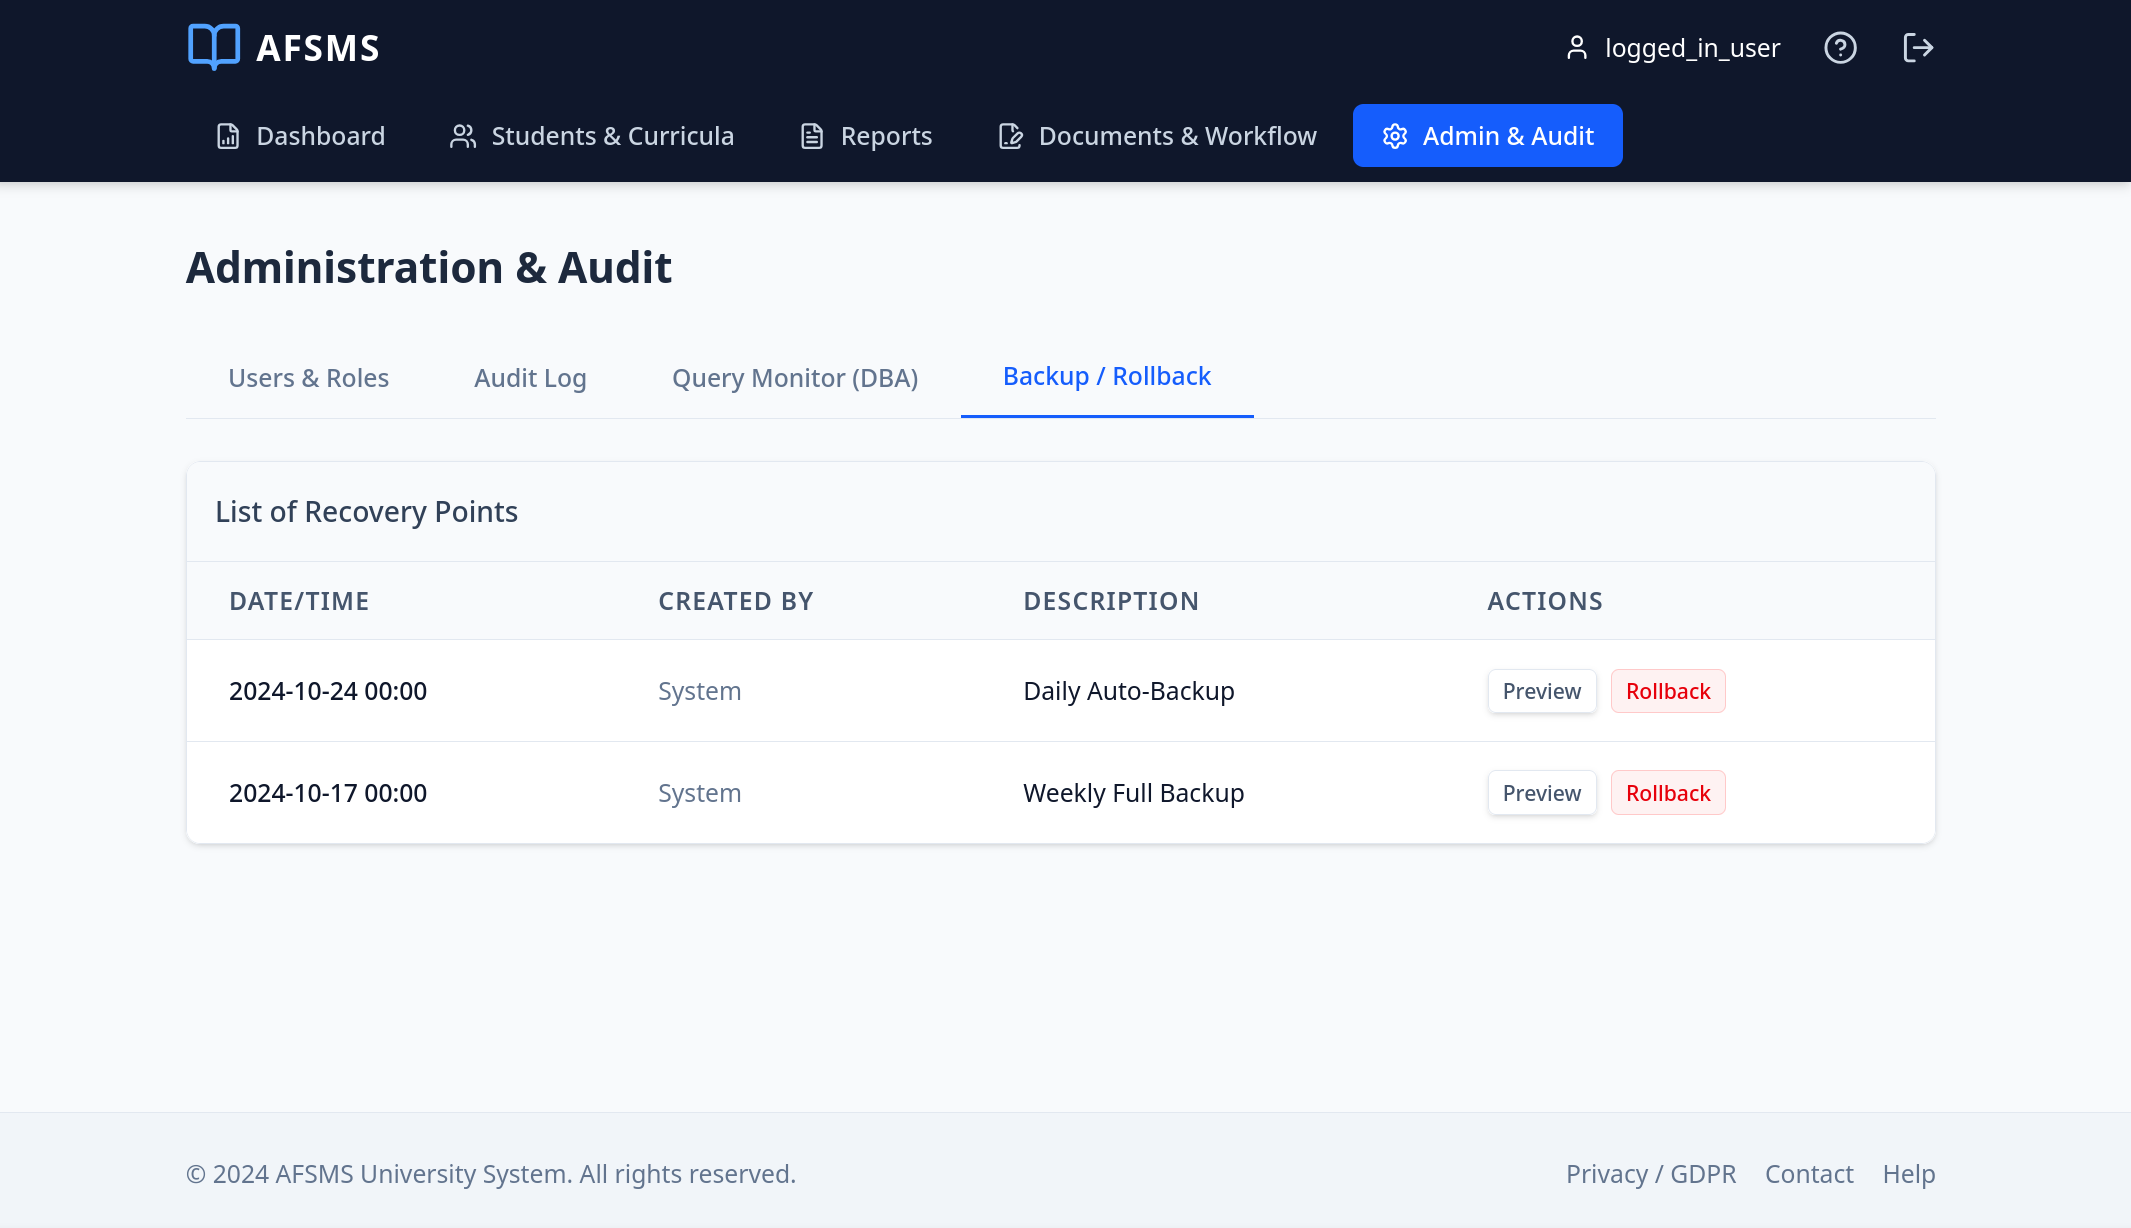
\includegraphics[width=\textwidth]{14.png}
        \caption{Rollback Point-in-Time Sequence Diagram.}
        \label{fig:img14}
    \end{minipage}
\end{figure}


\subsection{Hardware Interfaces}
AFSMS is a browser-based client-server system. Its hardware interfaces are defined by the server infrastructure and end-user devices (per IEEE 5.2.1.3 and IEEE 5.3.1).

\subsubsection{Server-Side Hardware Interface}
\begin{itemize}
    \item \textbf{Deployment:} Deployable on physical (on-premises) or virtualized servers supporting multi-threaded concurrent processing.
    \item \textbf{Storage:} Scalable primary and secondary storage for the operational database and long-term activity log retention (auditing and point-in-time recovery).
    \item \textbf{Network:} The server exposes the application over standard network interfaces (Ethernet/Wi-Fi via the institutional network).
\end{itemize}

\subsubsection{Client-Side Hardware Interface}
\begin{itemize}
    \item \textbf{Supported Devices:} Any internet-connected device with a modern browser --- desktop PCs, laptops, tablets, and smartphones.
    \item \textbf{Interaction:} Full-screen graphical UI within the browser; no legacy terminal interactions.
    \item \textbf{Peripherals:} No specialized hardware required (no barcode scanners or smart-card readers). Standard input only: keyboard and mouse on PCs/laptops; touch on mobile devices.
\end{itemize}

\subsubsection{Hardware-Related Configuration Characteristics}
\begin{itemize}
    \item \textbf{Ports:} Inbound TCP port 443 (HTTPS) required. All other service ports (e.g., database administration) restricted to internal network interfaces.
\end{itemize}

\subsubsection{Logical Characteristics of Hardware Interactions}
\begin{itemize}
    \item \textbf{Network Tolerance:} The server must handle up to 10,000 simultaneous TCP connections without packet loss during peak exam periods.
    \item \textbf{Network Latency:} Server routing must support round-trip latency under 100ms.
    \item \textbf{Storage I/O:} Database drives must deliver sufficient IOPS to process offline backups without locking the database or timing out user sessions.
\end{itemize}

\subsection{Software Interfaces}
This section defines the logical connections between AFSMS and external software components.

\subsubsection{Interfaces with External Applications}

\textbf{A. Data Persistence Interface (DBMS)}
\begin{itemize}
    \item \textbf{Purpose:} Persistent storage and retrieval of academic data and audit logs; supports point-in-time recovery and offline backups.
    \item \textbf{Inbound:} Query results for student records, curricula, grades, document metadata, user roles, and audit entries.
    \item \textbf{Outbound:} CUD (Create, Update, Delete) transactions for academic entities; append-only log events for all operations.
    \item \textbf{Format:} Relational records via SQL (JDBC/ODBC), including rollback recovery commands.
\end{itemize}

\textbf{B. Import and Export Interface (Microsoft Excel)}
\begin{itemize}
    \item \textbf{Inbound:} User-provided structured files (student lists, curricula) validated by the UI layer.
    \item \textbf{Outbound:} Report exports and tabular datasets (e.g., e-Grade Centralizer).
    \item \textbf{Format:} .XLSX, .XLS, .CSV, and .XML files. Column definitions and templates are documented.
\end{itemize}

\textbf{C. Communication and Workflow Interface (Microsoft Outlook)}
\begin{itemize}
    \item \textbf{Outbound:} Composed emails (recipients, subject, body) with optional attachments (PDF reports).
    \item \textbf{Inbound:} Basic delivery status (if supported by the API); primarily send-initiated.
    \item \textbf{Format:} Standard email fields via Microsoft Graph API or SMTP; attachments in PDF/XLS/CSV.
\end{itemize}

\textbf{D. Authentication Interface (University SSO)}
\begin{itemize}
    \item \textbf{Inbound:} Authentication assertions/tokens and unique user IDs after login.
    \item \textbf{Outbound:} Authentication requests and redirects to the SSO endpoint.
    \item \textbf{Format:} SAML assertions or OAuth2/OIDC tokens (implementation-dependent).
\end{itemize}

\textbf{E. Report Rendering Interface (PDF-Gen)}
\begin{itemize}
    \item \textbf{Inbound:} Compiled binary file for download or email attachment.
    \item \textbf{Outbound:} HTML or tabular data templates pushed to the rendering engine.
    \item \textbf{Format:} .PDF files conforming to ISO 32000.
\end{itemize}

\subsubsection{Shared Data and Constraints}
\begin{itemize}
    \item \textbf{Data Sharing:} The system exports structured academic datasets in .CSV, .XML, .XLS, and .PDF.
    \item \textbf{Authentication Restriction:} Authentication is constrained to the institutional SSO. A standalone credential database is prohibited by institutional security policy.
    \item \textbf{Transaction Integrity:} The DBMS must enforce strict transaction logging for every operation to guarantee point-in-time recovery (rollback).
\end{itemize}

\textbf{Software Component Summary:}
\begin{table}[H]
\centering
\small
\setlength{\arraystretch}{0.9}
\begin{tabularx}{\textwidth}{>{\raggedright\arraybackslash}p{1.8cm} >{\raggedright\arraybackslash}p{1.0cm} >{\raggedright\arraybackslash}p{1.8cm} >{\raggedright\arraybackslash}p{2.0cm} >{\raggedright\arraybackslash}X}
\toprule
\textbf{Software Component} & \textbf{Mnem.} & \textbf{Version / Standard} & \textbf{Source / Provider} & \textbf{Interface Purpose \& Data Formats} \\
\midrule
Relational Database & DBMS & 8.0.36 (MySQL) / 15+ (PostgreSQL) & University Data Center / Cloud & Store student data, curricula, and logs. Formats: SQL, JDBC/ODBC, Log files. \\
\midrule
Operating System & OS & Windows 11 Pro / Server 2022 & Local Infra. / Microsoft & Runtime environment for server and registrar workstations. \\
\midrule
Microsoft Excel & MS-XLS & 2016, 2019, 2021, 365 & Microsoft Corp. & Bulk data import and report export (e-Centralizer). Formats: .XLS, .CSV, .XML. \\
\midrule
Microsoft Outlook & MS-OUT & 2016, 2019, 2021, 365 & Microsoft Corp. & Document workflow management and group messaging. Formats: SMTP/MAPI, Microsoft Graph API. \\
\midrule
PDF Renderer & PDF-Gen & Implementa- tion Dependent & Third-party (iText/TCPDF) & Generate official documents (e-Transcript). Formats: .PDF. \\
\midrule
Auth Subsystem & SSO & SAML 2.0 / OAuth 2.0 & Univ. Security & Single Sign-On authentication. \\
\bottomrule
\end{tabularx}
\normalsize
\setlength{\arraystretch}{1.3}
\end{table}

\subsection{Communications Interfaces}
This section defines the communications protocols, message formatting, and security standards (per IEEE 5.2.1.5 and IEEE 5.3.1).

\subsubsection{Network and Web Server Communications}
All primary interactions occur over WAN or LAN, from the client web browser to the AFSMS web server.

\textbf{Protocols \& Standards:}
\begin{table}[H]
\begin{tabularx}{\textwidth}{>{\raggedright\arraybackslash}p{2.2cm} >{\raggedright\arraybackslash}p{2cm} >{\raggedright\arraybackslash}X}
\toprule
\textbf{Std./Prtcl.} & \textbf{Purpose} & \textbf{Notes} \\
\midrule
HTTPS (TLS 1.2+) & Secure Transport & All client-server traffic, including SSO exchanges. \\
\midrule
HTTP/1.1 or newer & Web Request Semantics & Unencrypted HTTP (Port 80) auto-redirects to HTTPS (Port 443). \\
\midrule
JSON & Structured Data & API responses and asynchronous operations. \\
\bottomrule
\end{tabularx}
\end{table}

\textbf{Security:}
All data in transit must be encrypted with modern TLS to protect student records, document workflows, and session tokens.

\subsubsection{Message Content, Formatting, and Commands}
\begin{itemize}
    \item \textbf{Client to Server:} HTTP requests (GET/POST) carrying form parameters, filter criteria, and search queries. File uploads use multipart/form-data.
    \item \textbf{Server to Client:} HTTP responses with tabular data and validation results, primarily as JSON payloads or binary file downloads.
    \item The UI layer must interpret standard HTTP status codes to display user-friendly error messages.
\end{itemize}

\subsubsection{Timing, Transfer Rates, and Synchronization}
\begin{itemize}
    \item \textbf{Synchronous:} General data entry and portal navigation provide real-time UI feedback.
    \item \textbf{Asynchronous:} Resource-intensive operations (bulk PDF generation, mass email) execute asynchronously with a polling mechanism or progress indicator to prevent UI blocking.
    \item \textbf{Transfer Rates:} Dependent on institutional bandwidth. Exact timeout thresholds and minimum transfer rates are TBD (detailed design phase), but must support the 3-minute usability benchmark (Section 2.1.2).
\end{itemize}

\subsubsection{E-mail and Document Workflow Communications}
\begin{itemize}
    \item \textbf{Source/Destination:} Initiated by the AFSMS server; delivered to the institutional Microsoft Exchange/Outlook server and ultimately to user inboxes.
    \item \textbf{Protocols:} Bulk group messages use the Microsoft Graph API (RESTful HTTPS) or SMTP.
    \item \textbf{Formatting:}
    \begin{itemize}
        \item Emails use the MIME standard (plain text and rich HTML).
        \item Workflow documents are transmitted as secure attachments in .pdf, .xls, or .csv format.
    \end{itemize}
\end{itemize}

\subsubsection{Data Export and Download Mechanisms}
\begin{itemize}
    \item \textbf{Protocols:} Exports download through the user's browser over HTTPS. No FTP/SFTP is required or permitted for end-user exports.
    \item \textbf{Formats:}
    \begin{itemize}
        \item CSV (Comma-Separated Values)
        \item XML (Extensible Markup Language)
        \item XLS/XLSX (Microsoft Excel Binary/OOXML)
        \item PDF (Portable Document Format)
    \end{itemize}
\end{itemize}


% --- SECTION 4: SYSTEM FEATURES ---
\section{System Features}
This section organizes AFSMS functional requirements by major system feature.

\subsection{Web Portal and Access Management}

\subsubsection{Description and Priority}
The web portal provides SSO-based authentication, user registration with an initial predefined rights set, and role-based access control across a public (unauthenticated) and private (authenticated) perspective.

\textbf{Priority:} High.

\subsubsection{Functional Requirements}
\begin{itemize}
    \item \textbf{REQ-AFSMS-01:} The system shall provide a public portal perspective accessible without authentication.
    \item \textbf{REQ-AFSMS-02:} The system shall provide a private portal perspective accessible only to authenticated users.
    \item \textbf{REQ-AFSMS-03:} The user interface shall be provided as a browser-based web interface.
    \item \textbf{REQ-AFSMS-04:} The system shall display data and query results in tabular form within the web page.
    \item \textbf{REQ-AFSMS-05:} The system shall enforce differentiated access to data based on user roles/rights in the private portal.
    \item \textbf{REQ-AFSMS-06:} The web interface shall be secure and shall provide differentiated access for different user roles.
    \item \textbf{REQ-AFSMS-07:} The system shall allow a user to register through the web interface.
    \item \textbf{REQ-AFSMS-08:} The system shall assign each newly registered user an initial predefined set of access rights.
    \item \textbf{REQ-AFSMS-09:} The system shall allow an authorized administrator to customize user access rights after registration.
    \item \textbf{REQ-AFSMS-10:} If registration input data is invalid, the system shall reject the request and display an error message.
    \item \textbf{REQ-AFSMS-11:} The system shall authenticate users using a single user account mechanism (SSO) for private portal access.
    \item \textbf{REQ-AFSMS-12:} The system's authentication mechanism shall conform to the security subsystem.
    \item \textbf{REQ-AFSMS-13:} If a user is not authenticated, the system shall deny access to the private portal perspective.
    \item \textbf{REQ-AFSMS-14:} The system shall enforce role-based access control for operations in the private portal.
    \item \textbf{REQ-AFSMS-15:} If a user attempts an operation without sufficient rights, the system shall block it and display an access-denied message.
\end{itemize}

\begin{figure}[htbp]
    \centering
    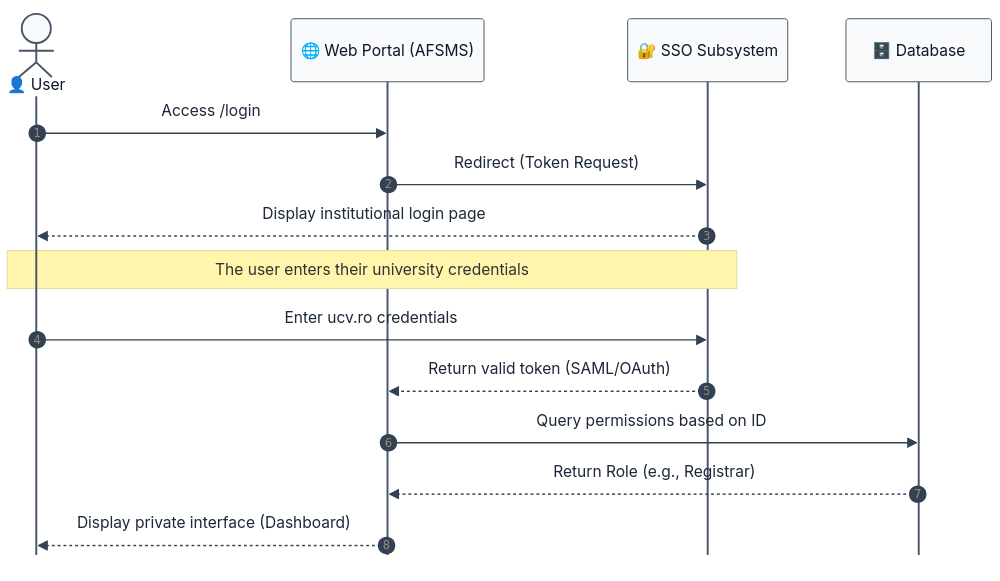
\includegraphics[width=0.9\textwidth]{2e.png}
    \caption{Web Portal and Access Management - SSO Authentication.}
    \label{fig:img2}
\end{figure}

\subsection{Academic Data Collection and Management}

\subsubsection{Description and Priority}
This module handles collection and management of curricula (study plans), study formations, and enrolled student data. It supports data extraction/import from databases, Excel files, and text files, with filters and transformations for database integration.

\textbf{Priority:} High.

\subsubsection{Functional Requirements}
\begin{itemize}
    \item \textbf{REQ-AFSMS-16:} The system shall allow collecting data for curricula (study plans), study formations, and their students.
    \item \textbf{REQ-AFSMS-17:} The system shall allow data collection and editing through the web interface.
    \item \textbf{REQ-AFSMS-18:} The system shall provide data extraction/import from databases, Excel files, and text files.
    \item \textbf{REQ-AFSMS-19:} The system shall provide filters and data transformations for integrating imported data into the system database.
    \item \textbf{REQ-AFSMS-20:} The system shall display managed academic data in tabular form within the web page.
    \item \textbf{REQ-AFSMS-21:} The system shall use selection lists to support easy visualization and localization of data.
    \item \textbf{REQ-AFSMS-22:} The system shall validate user-entered and imported data in the UI module and generate error messages for invalid inputs.
    \item \textbf{REQ-AFSMS-23:} For frequent validation errors, the system shall suggest resolution methods in error messages.
    \item \textbf{REQ-AFSMS-24:} The system shall support modifying existing academic data records, subject to the user's assigned rights.
\end{itemize}

\subsection{Reporting and Export}

\subsubsection{Description and Priority}
The reporting module allows authorized users to generate academic reports (including the e-Grade Centralizer by specialization, year, and form of education with students in alphabetical order) and export them in CSV, XML, XLS, and PDF formats.

\textbf{Priority:} High.

\subsubsection{Functional Requirements}
\begin{itemize}
    \item \textbf{REQ-AFSMS-25:} The system shall include a reporting module.
    \item \textbf{REQ-AFSMS-26:} The system shall allow authorized users to generate reports in accordance with their allocated rights.
    \item \textbf{REQ-AFSMS-27:} The system shall generate the e-Grade Centralizer at the level of specialization, year of study, and form of education.
    \item \textbf{REQ-AFSMS-28:} The system shall list students in alphabetical order within the e-Grade Centralizer report.
    \item \textbf{REQ-AFSMS-29:} The reporting component shall allow saving/exporting reports in CSV, XML, XLS, and PDF formats.
    \item \textbf{REQ-AFSMS-30:} The system shall display generated reports in tabular form in the web interface.
    \item \textbf{REQ-AFSMS-31:} If a user attempts to generate or export a report without sufficient rights, the system shall block the operation and display an access-denied message.
    \item \textbf{REQ-AFSMS-32:} If report parameters are missing or invalid, the system shall reject the request and display an error message.
\end{itemize}

\begin{figure}[htbp]
    \centering
    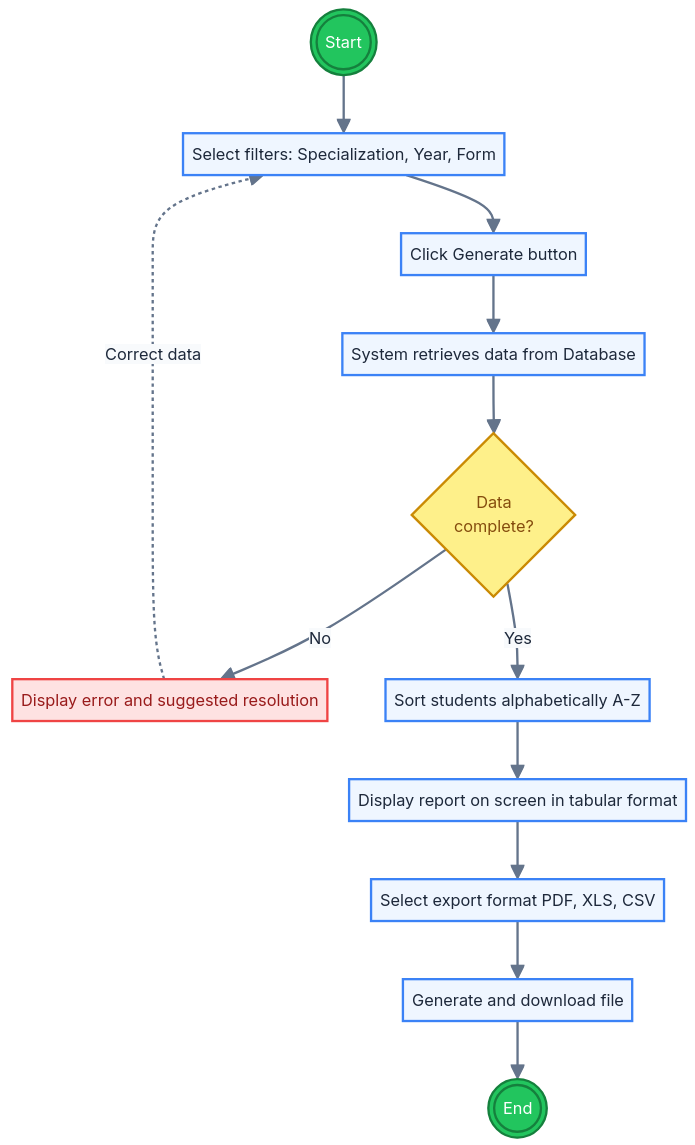
\includegraphics[width=0.9\textwidth, height=0.9\textheight, keepaspectratio]{3e.png}
    \caption{Reporting and Export - e-Grade Centralizer.}
    \label{fig:img3}
\end{figure}

\subsection{Document Workflow and Search}

\subsubsection{Description and Priority}
The system provides document workflow management for the faculty secretariat, supporting electronic circulation of documents for information, approval, or modification, as well as electronic storage and retrieval. Document search is available by file type, creation date, author, and document content.

\textbf{Priority:} Medium-High.

\subsubsection{Stimulus/Response Sequences}
\begin{table}[H]
\begin{tabularx}{\textwidth}{>{\raggedright\arraybackslash}p{3.2cm} >{\raggedright\arraybackslash}X}
\toprule
\textbf{Stimulus} & \textbf{Response} \\
\midrule
An authenticated user opens the Document Management module. & The system displays the document workspace with document list and available actions. \\
\midrule
The user submits/forwards a document for information, approval, or modification. & The system records the workflow action and updates the document's state. \\
\midrule
The user searches for a document by file type. & The system returns matching documents. \\
\midrule
The user searches by creation date and/or author. & The system returns documents matching the metadata criteria. \\
\midrule
The user searches by content. & The system returns documents matching the content query. \\
\midrule
The user opens a document from search results. & The system retrieves and displays/downloads it per the user's rights. \\
\midrule
The user provides invalid search criteria. & The system rejects the search and displays an error message. \\
\bottomrule
\end{tabularx}
\end{table}

\subsubsection{Functional Requirements}
\begin{itemize}
    \item \textbf{REQ-AFSMS-33:} The system shall support document workflow management within the faculty secretariat.
    \item \textbf{REQ-AFSMS-34:} The system shall support electronic circulation of documents for information, approval, or modification.
    \item \textbf{REQ-AFSMS-35:} The system shall support electronic storage and retrieval of documents.
    \item \textbf{REQ-AFSMS-36:} The system shall allow searching documents by file type.
    \item \textbf{REQ-AFSMS-37:} The system shall allow searching documents by creation date.
    \item \textbf{REQ-AFSMS-38:} The system shall allow searching documents by author.
    \item \textbf{REQ-AFSMS-39:} The system shall allow searching documents by document content.
    \item \textbf{REQ-AFSMS-40:} The system shall restrict document access and workflow actions according to the user's assigned rights.
    \item \textbf{REQ-AFSMS-41:} If search input criteria is invalid, the system shall reject the search and display an error message.
\end{itemize}

\begin{figure}[htbp]
    \centering
    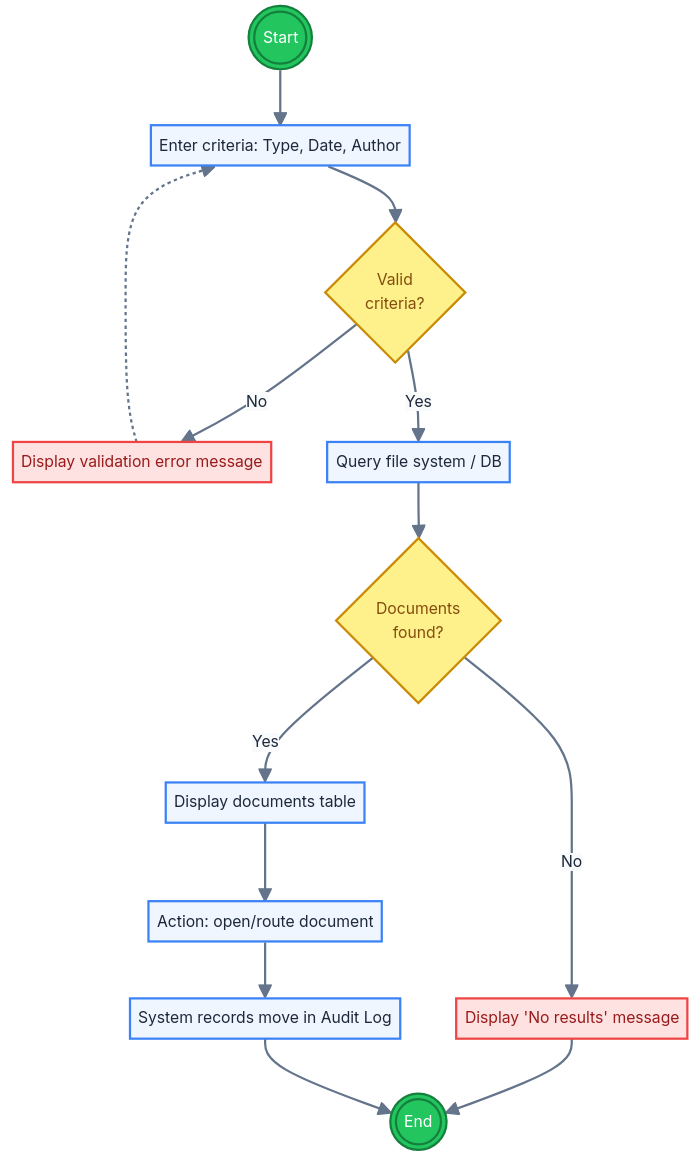
\includegraphics[width=0.9\textwidth]{4e.png}
    \caption{Document Workflow and Search - Management Interface.}
    \label{fig:img4}
\end{figure}

\subsection{User Groups and Messaging}

\subsubsection{Description and Priority}
The system allows defining user groups and executing group-level operations, including sending email messages to all group members via Microsoft Outlook integration.

\textbf{Priority:} Medium.

\subsubsection{Functional Requirements}
\begin{itemize}
    \item \textbf{REQ-AFSMS-42:} The system shall allow defining user groups.
    \item \textbf{REQ-AFSMS-43:} The system shall allow executing operations at group level.
    \item \textbf{REQ-AFSMS-44:} The system shall allow sending email messages to all members of a user group.
    \item \textbf{REQ-AFSMS-45:} The system shall support integration with Microsoft Outlook for messaging/communication functions.
    \item \textbf{REQ-AFSMS-46:} The system shall restrict group management and group operations according to the user's assigned rights.
\end{itemize}

\subsection{Validation and Error Handling}

\subsubsection{Description and Priority}
The system validates user-entered data in the UI module, generates clear error messages for invalid inputs, and suggests resolution methods for frequent error cases.

\textbf{Priority:} High.

\subsubsection{Functional Requirements}
\begin{itemize}
    \item \textbf{REQ-AFSMS-47:} The system shall validate user-entered data within the UI module.
    \item \textbf{REQ-AFSMS-48:} If input data is invalid, the system shall reject the input and display an error message.
    \item \textbf{REQ-AFSMS-49:} For frequent validation error cases, the system shall suggest resolution methods in error messages.
    \item \textbf{REQ-AFSMS-50:} The system shall prevent saving or submitting invalid data to the database.
\end{itemize}

\subsection{Audit Logging and Data Recovery}

\subsubsection{Description and Priority}
The system records all executed operations in activity logs containing the acting user and relevant data details. It provides rollback capability to return to previous data states and supports database-level point-in-time recovery and offline backups.

\textbf{Priority:} High.

\subsubsection{Stimulus/Response Sequences}
\begin{table}[H]
\begin{tabularx}{\textwidth}{>{\raggedright\arraybackslash}p{3.2cm} >{\raggedright\arraybackslash}X}
\toprule
\textbf{Stimulus} & \textbf{Response} \\
\midrule
A user performs an operation (create/update/ delete/import/ export/report generation). & The system records the operation in the activity log with the acting user and relevant details. \\
\midrule
An administrator reviews system activity. & The system provides access to log records for monitoring and audit (subject to rights). \\
\midrule
An administrator triggers rollback to a previous state. & The system restores data to the selected state and confirms completion. \\
\midrule
A rollback operation completes. & The system records the rollback as a logged activity. \\
\midrule
Point-in-time recovery is requested at database level. & The system restores data to the specified time point, consistent with backups/logs. \\
\midrule
Offline backup is scheduled or triggered. & The system produces an offline backup usable for recovery. \\
\bottomrule
\end{tabularx}
\end{table}

\subsubsection{Functional Requirements}
\begin{itemize}
    \item \textbf{REQ-AFSMS-51:} The system shall record all executed operations.
    \item \textbf{REQ-AFSMS-52:} For each logged activity, the system shall store the user identity that performed the action.
    \item \textbf{REQ-AFSMS-53:} For each logged activity, the system shall store relevant details about the accessed/modified data.
    \item \textbf{REQ-AFSMS-54:} The system shall provide rollback capability to return to previous data states to prevent/correct data collection errors.
    \item \textbf{REQ-AFSMS-55:} The system/database shall support recovery of data to a specified point in time.
    \item \textbf{REQ-AFSMS-56:} The system/database shall support offline backup to enable data recovery.
    \item \textbf{REQ-AFSMS-57:} The system shall restrict access to logs and rollback/recovery operations according to assigned rights.
\end{itemize}

\begin{figure}[htbp]
    \centering
    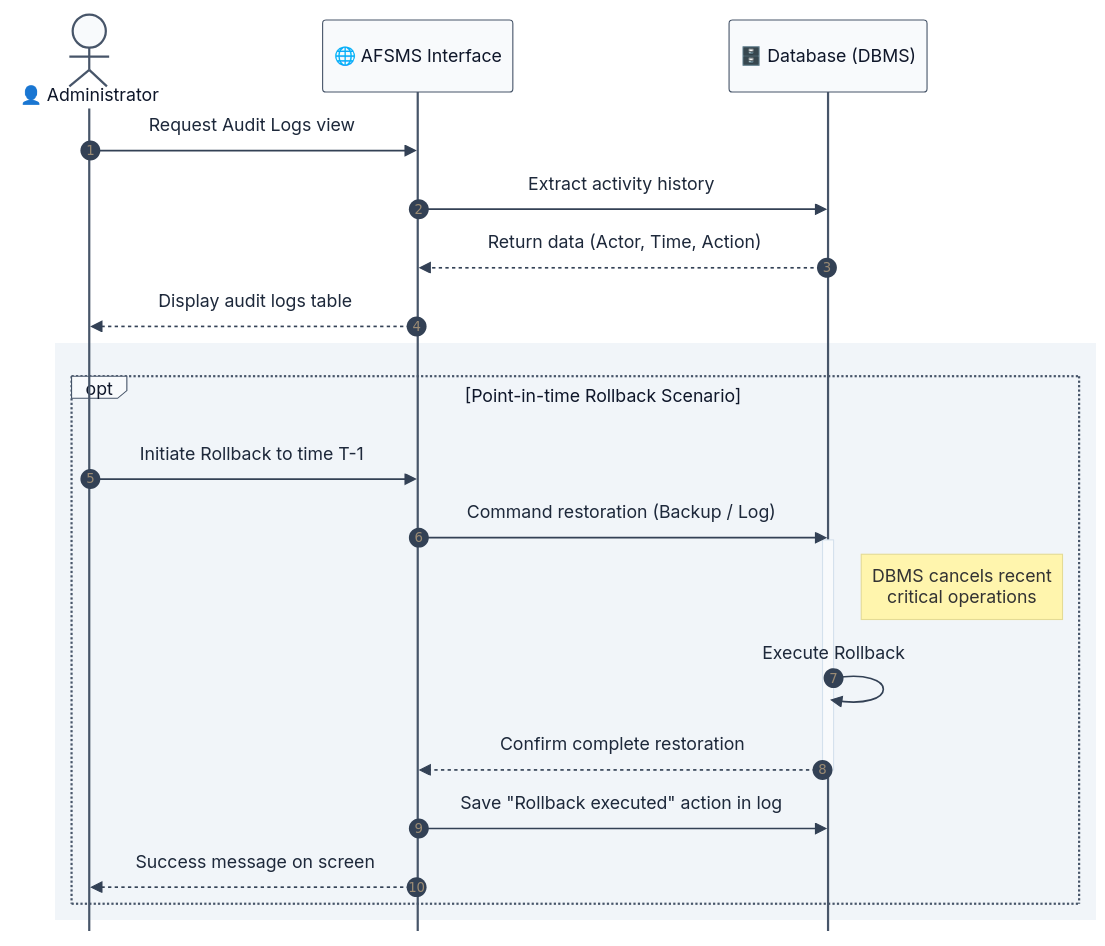
\includegraphics[width=0.9\textwidth]{5e.png}
    \caption{Audit Logging and Data Recovery - Rollback.}
    \label{fig:img5}
\end{figure}

% --- SECTION 5: OTHER NONFUNCTIONAL REQUIREMENTS ---
\section{Other Nonfunctional Requirements}

\subsection{Performance Requirements}
This section specifies measurable performance constraints for AFSMS under normal and peak workloads. All performance requirements use the ID format NFR-AFSMS-PERF-XX for traceability.

\subsubsection{Capacity (Static numerical requirements)}
\begin{itemize}
    \item \textbf{NFR-AFSMS-PERF-01:} The system shall support web-based access for all user interactions without requiring special client hardware or software beyond a standard web browser.
    \item \textbf{NFR-AFSMS-PERF-02:} The database shall support managing a large volume of academic data (including historical growth).
    \item \textbf{NFR-AFSMS-PERF-03:} The system shall support concurrent user access to database information.
    \item \textbf{NFR-AFSMS-PERF-04:} The DBMS shall support web-based administration, concurrent access, and query monitoring.
    \item \textbf{NFR-AFSMS-PERF-05 (TBD):} The system shall support at least TBD simultaneous authenticated users and at least TBD total stored academic records/documents, measured in a production-like environment.
\end{itemize}

\subsubsection{Response time and throughput (Dynamic numerical requirements)}
Where feasible, dynamic targets are expressed as percentiles tied to workload and dataset size.
\begin{itemize}
    \item \textbf{NFR-AFSMS-PERF-06 (TBD):} For interactive portal actions (open module page, load tabular view), 95\% of requests shall complete in $\leq$ TBD seconds under normal workload.
    \item \textbf{NFR-AFSMS-PERF-07 (TBD):} For dataset listing via selection lists, 95\% of requests shall complete in $\leq$ TBD seconds under normal workload (dataset up to TBD rows).
    \item \textbf{NFR-AFSMS-PERF-08 (TBD):} Document search requests (by file type, date, author, or content) shall return results in $\leq$ TBD seconds for 95\% of queries (repository up to TBD documents).
    \item \textbf{NFR-AFSMS-PERF-09 (TBD):} Report generation (including the e-Grade Centralizer) shall complete in $\leq$ TBD seconds for 95\% of requests (up to TBD students, normal workload).
    \item \textbf{NFR-AFSMS-PERF-10 (TBD):} Report export shall complete in $\leq$ TBD seconds for 95\% of requests per format (CSV, XML, XLS, PDF; up to TBD rows).
\end{itemize}

\subsubsection{Background operations and recovery performance}
\begin{itemize}
    \item \textbf{NFR-AFSMS-PERF-11 (TBD):} Offline backups shall be schedulable and shall not cause visible downtime exceeding TBD minutes during planned windows.
    \item \textbf{NFR-AFSMS-PERF-12 (TBD):} Point-in-time recovery and rollback shall complete within TBD for the standard recovery scenario (TBD dataset size).
\end{itemize}

\subsubsection{Performance measurement conditions (Verification)}
\begin{itemize}
    \item \textbf{NFR-AFSMS-PERF-13:} Each performance requirement shall be verified in a controlled environment, documented with: workload type, concurrent users, dataset size, and network conditions.
    \item \textbf{NFR-AFSMS-PERF-14:} Performance requirements shall be validated through dedicated performance tests.
\end{itemize}

\subsection{Safety Requirements}
This section defines requirements to prevent loss, corruption, or irreversible modification of critical data. Safety requirements use IDs NFR-AFSMS-SAFE-XX.

\subsubsection{Data integrity and loss prevention}
\begin{itemize}
    \item \textbf{NFR-AFSMS-SAFE-01:} The system shall record all operations to support auditing and incident investigation.
    \item \textbf{NFR-AFSMS-SAFE-02:} The system shall provide rollback capability to previous data states to prevent or correct collection errors.
    \item \textbf{NFR-AFSMS-SAFE-03:} The database shall support point-in-time recovery to a specified time.
    \item \textbf{NFR-AFSMS-SAFE-04:} The database shall support offline backup for recovery after failures.
    \item \textbf{NFR-AFSMS-SAFE-05:} Rollback/recovery operations shall be controlled and their completion recorded as audited activities.
\end{itemize}

\subsubsection{Safe input and validation safeguards}
\begin{itemize}
    \item \textbf{NFR-AFSMS-SAFE-06:} The system shall validate user-entered data in the UI module before persistence.
    \item \textbf{NFR-AFSMS-SAFE-07:} On validation failure, the system shall display error messages and suggest resolutions for frequent error cases.
    \item \textbf{NFR-AFSMS-SAFE-08:} The system shall prevent saving invalid data to the database.
\end{itemize}

\subsubsection{Controlled execution of critical actions}
\begin{itemize}
    \item \textbf{NFR-AFSMS-SAFE-09:} The system shall enforce role-based access to data and operations to prevent unauthorized actions.
    \item \textbf{NFR-AFSMS-SAFE-10:} The system shall restrict access to logs, rollback, and recovery functions by user rights.
    \item \textbf{NFR-AFSMS-SAFE-11:} Only authenticated users shall access the private portal where data modifications and report generation occur.
\end{itemize}

\subsubsection{Safety-related operational constraints}
\begin{itemize}
    \item \textbf{NFR-AFSMS-SAFE-12:} The system shall support safe concurrent access to avoid data corruption under multi-user usage.
    \item \textbf{NFR-AFSMS-SAFE-13:} The system shall log the acting user identity and relevant data details for each activity to enable accountability and rollback targeting.
\end{itemize}

\subsubsection{Verification (Safety)}
\begin{itemize}
    \item \textbf{NFR-AFSMS-SAFE-14:} Backup, rollback, and recovery requirements shall be verified through dedicated recovery test scenarios (e.g., introduce a controlled error, then demonstrate restoration).
    \item \textbf{NFR-AFSMS-SAFE-15:} Input validation requirements shall be verified through negative test cases covering invalid formats, missing fields, and frequent error patterns.
\end{itemize}

\subsection{Security Requirements}
This section defines security and privacy requirements for protecting academic data and controlling access. Security requirements use IDs NFR-AFSMS-SEC-XX.

\subsubsection{Authentication and session access control}
\begin{itemize}
    \item \textbf{NFR-AFSMS-SEC-01:} The system shall provide a secure web interface with access differentiated by user role/rights.
    \item \textbf{NFR-AFSMS-SEC-02:} The portal shall have two perspectives: public (unauthenticated) and private (registered users only).
    \item \textbf{NFR-AFSMS-SEC-03:} The system shall require authentication for any action that modifies data, generates private reports, or accesses private records.
    \item \textbf{NFR-AFSMS-SEC-04:} The authentication mechanism shall comply with the institution's centralized security subsystem for unified account-based login.
\end{itemize}

\subsubsection{Authorization (least privilege)}
\begin{itemize}
    \item \textbf{NFR-AFSMS-SEC-05:} The system shall enforce authorization checks for each protected operation (create, update, delete, report generation, document workflow) based on the user's assigned rights.
    \item \textbf{NFR-AFSMS-SEC-06:} The system shall allow defining users and user groups with different access rights and enforce them across all modules.
    \item \textbf{NFR-AFSMS-SEC-07:} Students shall only access data permitted by their rights and the system shall prevent access to other students' records.
\end{itemize}

\subsubsection{Secure communications and transport protection}
\begin{itemize}
    \item \textbf{NFR-AFSMS-SEC-08:} The system shall use HTTPS for all browser-server communication to protect authentication and academic data in transit.
\end{itemize}

\subsubsection{Auditability and accountability}
\begin{itemize}
    \item \textbf{NFR-AFSMS-SEC-09:} The system shall log all activities, identifying the acting user and relevant details of accessed/modified information.
    \item \textbf{NFR-AFSMS-SEC-10:} The system shall retain sufficient audit information to support investigation of unauthorized access and recovery/rollback targeting.
\end{itemize}

\subsubsection{Privacy and regulatory constraints}
\begin{itemize}
    \item \textbf{NFR-AFSMS-SEC-11:} The system shall comply with GDPR for personal student data and with university policies for academic data retention.
    \item \textbf{NFR-AFSMS-SEC-12:} Example data in documentation, training, or prototypes shall be anonymized/synthetic with no real student data.
\end{itemize}

\subsubsection{Security verification requirements}
\begin{itemize}
    \item \textbf{NFR-AFSMS-SEC-13:} Authentication and role-based authorization shall be verified via test cases that attempt restricted access with insufficient rights (expected: access denied and logged).
    \item \textbf{NFR-AFSMS-SEC-14:} Audit logging shall be verified by confirming each critical action produces a log entry with actor identity and action context.
\end{itemize}

\subsection{Software Quality Attributes}
This section specifies quality characteristics beyond performance, safety, and security. Functional behavior (what the system does) is covered in Section 4; this section addresses how well it does it.

\subsubsection{Maintainability and extensibility}
\begin{itemize}
    \item \textbf{NFR-AFSMS-QUAL-09:} The architecture shall be extensible so new modules can be added without negatively affecting existing functionality.
    \item \textbf{NFR-AFSMS-QUAL-10 (TBD):} The project shall define module-level boundaries for core capabilities (data collection, reporting, logging) to maintain the system as modules evolve.
\end{itemize}

\subsubsection{Portability and compatibility}
\begin{itemize}
    \item \textbf{NFR-AFSMS-QUAL-11:} The system shall be platform-agnostic on the client side, relying on standard web technologies with no local installation required.
    \item \textbf{NFR-AFSMS-QUAL-12:} The system shall coexist with Microsoft Excel and Outlook on registrar workstations.
\end{itemize}

\subsection{Business Rules}
Business rules define operational principles (who can do what, under which conditions) enforced through role-based access and workflow constraints.
\begin{itemize}
    \item \textbf{BR-AFSMS-01:} The Web Portal shall have a Public area (any user) and a Private area (registered users only).
    \item \textbf{BR-AFSMS-02:} Only authenticated Private-area users may modify data or generate internal reports; allowed actions depend on assigned rights.
    \item \textbf{BR-AFSMS-03:} New users receive an initial predefined set of rights, customizable afterward for differentiated access.
    \item \textbf{BR-AFSMS-04:} Academic data must display in tabular form to support administrative workflows.
    \item \textbf{BR-AFSMS-05:} Data entry and lookup shall use selection lists (dropdowns) to reduce errors.
    \item \textbf{BR-AFSMS-06:} The e-Grade Centralizer shall be produced by specialization, study year, and form of education, with students in alphabetical order.
    \item \textbf{BR-AFSMS-07:} Reports shall be exportable in CSV, XML, XLS, and PDF.
    \item \textbf{BR-AFSMS-08:} Document search shall support file type, creation date, author, and content (keyword) criteria.
    \item \textbf{BR-AFSMS-09:} The system shall allow defining user groups and group-level operations, including group email.
    \item \textbf{BR-AFSMS-10:} All operations shall be logged with user identity and relevant data details.
    \item \textbf{BR-AFSMS-11:} The system shall support rollback/recovery to previous data states.
    \item \textbf{BR-AFSMS-12:} The database shall support offline backup and point-in-time recovery as part of operational maintenance.
\end{itemize}

\subsection{Coding Standards and Code Quality Requirements}
The following coding standards shall be respected during system development to ensure maintainable and high-quality source code.
\begin{itemize}
    \item \textbf{CODE-01:} All source code shall follow consistent naming conventions: classes in PascalCase and variables in camelCase.
    \item \textbf{CODE-02:} Each function shall implement a single responsibility and should not exceed 50 lines of code where possible.
    \item \textbf{CODE-03:} Code duplication shall be avoided; reusable functionality shall be placed in shared modules.
    \item \textbf{CODE-04:} All public classes and methods shall include documentation comments describing their purpose and parameters.
    \item \textbf{CODE-05:} Error handling shall be implemented for all operations interacting with external systems or files.
    \item \textbf{CODE-06:} Hard-coded values (``magic numbers'') shall be avoided; constants shall be defined in configuration files or constant definitions.
    \item \textbf{CODE-07:} Source code shall be structured in logical modules corresponding to system components.
    \item \textbf{CODE-08:} All code shall be reviewed through peer code review before integration into the main branch.
    \item \textbf{CODE-09:} Static code analysis tools shall be used to detect potential bugs and code smells.
    \item \textbf{CODE-10:} Unit tests shall be implemented for core business logic components.
\end{itemize}


% --- SECTION 6: OTHER REQUIREMENTS ---
\section{Other Requirements}

\subsection{Database Requirements}
\begin{itemize}
    \item \textbf{Data Retention:} Student academic records (e-Transcripts) shall be maintained indefinitely per educational legislation. System audit logs may be archived after 5 years.
    \item \textbf{Relational Integrity:} Curriculum modifications must not retroactively alter previously validated grades in the e-Grade Centralizer.
\end{itemize}

\subsection{Legal and Regulatory Requirements}
\begin{itemize}
    \item \textbf{GDPR Compliance:} All processing of PII (student names, identification numbers) must comply with EU/Romanian GDPR.
    \item \textbf{Anonymization:} Sample data for documentation or training must be synthetic with no real student information.
\end{itemize}

\subsection{Internationalization and Localization}
\begin{itemize}
    \item \textbf{Language Support:} The public portal shall support both Romanian and English for international students and mobility programs.
    \item \textbf{Character Encoding:} All components (including PDF and Excel exports) must use UTF-8 encoding for correct rendering of Romanian diacritics.
\end{itemize}

% --- APPENDICES ---
\newpage
\appendix

\section{Glossary}
\begin{itemize}
    \item \textbf{AFSMS (Automated Faculty Student Management System):} The software product specified here, designed to automate administration of student records, curricula, and document circulation within a university faculty.
    \item \textbf{e-Registrul matricol (e-Transcript):} A secure electronic document recording a student's full academic history --- all completed disciplines, contact hours, and ECTS credits.
    \item \textbf{e-Centralizatorul de note (e-Grade Centralizer):} A standardized electronic report aggregating student exam results within an academic year, organized by specialization and study formation.
    \item \textbf{Managementul fluxului de documente (Document Workflow Management):} The system capability for electronic routing, tracking, and storage of administrative documents for information, approval, or modification.
    \item \textbf{Rollback:} A data integrity function enabling the database to revert to a previously verified stable state, neutralizing data corruption or collection errors.
\end{itemize}

\section{Analysis Models}
This appendix provides logical models illustrating AFSMS functional requirements and data relationships.

\subsection{High-Level System Context Diagram}
The Context Diagram defines the AFSMS boundary and its external entities:
\begin{itemize}
    \item \textbf{AFSMS Core System:} Processes academic requests, report generation, and document workflows.
    \item \textbf{External Entities:}
    \begin{itemize}
        \item \textit{Registrar/Secretariat Staff:} Provide student data, curricula updates, and document routing.
        \item \textit{Teaching Staff (Professors):} Provide examination results and grades.
        \item \textit{Students:} Receive academic standings, schedules, and grade reports.
        \item \textit{University SSO Subsystem:} Provides authentication tokens.
        \item \textit{Microsoft Ecosystem:} Facilitates Excel import/export and Outlook communications.
    \end{itemize}
\end{itemize}

\subsection{Data Flow Diagram (DFD Level 0)}
Primary data transformations:
\begin{enumerate}
    \item \textbf{Data Collection:} Accepts raw data from external files (Excel, text) and databases, applies transformations and filters for system integration.
    \item \textbf{Report Processing:} Transforms stored academic records (grades, ECTS, hours) into standardized formats (e-Grade Centralizer, e-Transcript).
    \item \textbf{Audit \& Log Generation:} Generates a log entry for every interaction, identifying the user and data modification for safety and rollback.
    \item \textbf{Workflow Management:} Directs electronic document circulation within the secretariat for approval or modification.
\end{enumerate}

\subsection{Entity-Relationship Model (Conceptual)}
Fundamental data structures and relationships:
\begin{itemize}
    \item \textbf{STUDENT:} Uniquely identified by personal details; enrolled in a STUDY FORMATION.
    \item \textbf{CURRICULUM (Plan de învățământ):} Defines DISCIPLINES, ECTS credits, and contact hours for a specialization.
    \item \textbf{GRADE:} Links a STUDENT to a DISCIPLINE for a specific academic year.
    \item \textbf{USER ACCOUNT:} Mapped to ROLES and PRIVILEGES for differentiated private portal access.
    \item \textbf{LOG ENTRY:} Append-only record linked to a USER ACCOUNT and an OPERATION.
\end{itemize}

\subsection{High-Level System States}
AFSMS has two primary logical states:
\begin{itemize}
    \item \textbf{Public Portal State:} Default state where visitors browse unauthenticated data (curricula, announcements).
    \item \textbf{Private Portal State:} Activated on successful SSO authentication. Provides differentiated services (Data Management, Reporting, Rollback) based on the user's role (Student, Professor, Registrar).
\end{itemize}

\section{To Be Determined List}
\begin{itemize}
    \item \textbf{TBD-1 (NFR-AFSMS-PERF-005):} Exact number of simultaneous authenticated users the server must support (estimated from university data center capacity).
    \item \textbf{TBD-2 (NFR-AFSMS-PERF-010--014):} Maximum time thresholds (in seconds) for loading tabular pages and generating PDF/XLS reports.
    \item \textbf{TBD-3 (Section 3.4.3):} Minimum data transfer rates and timeout thresholds for institutional network requests.
    \item \textbf{TBD-4 (NFR-AFSMS-QUAL-010):} Exact module boundaries to ensure extensibility without negative effects.
    \item \textbf{TBD-5 (Section 3.3.4):} Specific version of the third-party PDF rendering library (e.g., iText or TCPDF).
\end{itemize}

\end{document}
